\documentclass[a4j,12pt]{jreport}
%\usepackage[dvips]{graphicx}
\usepackage[dvipdfmx]{graphicx}%pdfの図を用いるため
\usepackage{mythesis}
\usepackage{multirow}
\usepackage{here}
\usepackage{url}%urlを使いたい
\usepackage{here}%図の位置を固定するために(文字と入れ替わらないように)
\usepackage{comment}
%\renewcommand{\abstractname}{abstract}

\setlength{\itemsep}{-1zh}
\title{
船舶の運航状況予測\\
Forecasting vessel operations
}
\icon{
		
\includegraphics[width=60mm,bb=0 0 550 550]{fig/ryukyu.pdf}
	}
\year{令和2年度 卒業論文}

%公開暗号方式を用いたSSH認証によるアカウント作成の簡略化\\
%Simplify Creating account by \\
%SSH authentication using public-key cryptography

\belongto{琉球大学工学部工学科知能情報コース}
\author{175755F 大城紳之亮  \\ 指導教員 {當間愛晃} }
%%
%% プリアンブルに記述
%% Figure 環境中で Table 環境の見出しを表示・カウンタの操作に必要
%%
\makeatletter
\newcommand{\figcaption}[1]{\def\@captype{figure}\caption{#1}}
\newcommand{\tblcaption}[1]{\def\@captype{table}\caption{#1}}
\makeatother
\setlength\abovecaptionskip{0pt}

\begin{document}

% タイトル
\maketitle
\baselineskip 17pt plus 1pt minus 1pt

\pagenumbering{roman}
\setcounter{page}{0}
%要旨は論文全体の要約です。予測するという話だけではなく結果、考察、今後の課題も述べよう。日本語でもいいです。あと書く場所は目次の前にしよう。
\begin{abstract}
 近年、地球温暖化等の影響により台風や異常気象など天候の変化が激しく、これらの天候の変化は、船舶の運航に支障をきたす。船舶の欠航情報は出航当日にしか発表されないため、利用者が今後のスケジュールを計画する際に支障が出る可能性がある。本研究では,気象予報図,気象データ,欠航データを用いて,機械学習を適用して運航予測を行うことでスケジュール組み立ての一助となることを目指す。本研究で対象とした八重山諸島周辺の航路の欠航データと気象画像、気象値をそれぞれ別のデータセットとして構築し、教師データと特徴量を日付別にスライドさせ航路ごとにモデルを作成した。数値モデルの実験結果において、散布図を確認することでモデルの重要視している特徴を確認できた。画像モデルでの実験結果では、どのような画像がモデルに対して影響を与えているか示した。また、特定の航路での精度評価から画像の周期性があることが明らかになった。今後の課題として、データセットの作成、モデルにおいて数値、画像の特徴を考慮する必要がある。
\end{abstract} 

\tableofcontents	% 目次
\listoffigures		% 図目次
\listoftables		% 表目次

%以下のように、章ごとに個別の tex ファイルを作成して、
% main.tex をコンパイルして確認する。
%章分けは個人で違うので下のフォーマットを参考にして下さい。
\renewcommand{\abstractname}{abstract}



% はじめに
%\documentclass[12pt]{jarticle}



\chapter{はじめに}
\label{chap:introduction}
\pagenumbering{arabic}


%序論の目安としては1枚半ぐらい.
%英語発表者は,最終予稿の「はじめに」の英訳などを載せてもいいかも.



\section{背景と目的}
近年、地球温暖化等の影響で台風や異常気象など天候の変化が激しい\cite{earth}。これらの天候変化は船舶の運航状況に支障をきたす。運航状況への支障として、船舶利用者が利用したいときに運航できない場合や貨物を運ぶ際に予定通りに運ぶことができないということがある。なかでも、旅客船に考えられる被害として、突然の欠航により船舶利用者の予定に支障が出る可能性がある。それにより経済的損失が発生する問題があると考えられる。船舶の運航を決定づける権限を持つのは船長であり、自身の経験に基づき気象通報、水路通報その他の航海に必要な情報を参考にすることで運航当日に決定している\cite{stan}。筆者は当日にしか公表されない船舶の運航状況を数日前に予測することで観光客や船舶の利用者のスケジュール組立ての一助を目指す。
関連研究として沿岸波浪および、船体運動データを用いたシミュレーションによる新たな欠航判断基準を提供するものがある\cite{Related-Research1}。この研究では船体運動などのデータが必要不可欠であり、そのデータを取得するのは簡単ではないため、データ取得の容易な気象状況の値、あるいは予報図から船舶の欠航を予測したいと考えた。本研究では機械学習を用い、過去の欠航データ、気象データを活用し数日先までの欠航を予測することを目的とし実験を行う。

\section{関連研究}
\subsection{欠航判断においての研究事例}
笹\cite{Related-Research1}らは運航判断において航海中の波浪の角度、周期が反映された船体運動にて評価すべきと考えている。そのため台風接近時のフェリーを検証対象とし船体運動データを観測した。また沿岸波浪(ナウファス)\cite{nowphas}と観測データをもとに船体運動のシミュレーションを実施し、検証した。これらの結果からフェリー欠航の新たな判断基準を提案するための基礎的研究を行った。
\\ 問題点として船体運動の縦揺れの再現結果が実測値よりも過小評価していることが挙げられる。シミュレーションの再現結果では船体の実際の有義振幅が6.76°であるのに対し計算結果では2.61°と半分以下の値が出力されている。有義振幅とは、ある地点で観測された連続値のデータの大きい方から全体の$1/3$の個数を平均して計算した振幅となる。また、シミュレーションに使用するデータが船体を観測して得られるデータのため、様々なフェリー航路への応用が難しく、データの取得が容易でない。そのため本研究では、データ取得が比較的容易である天気予報webサイトなwindy\cite{windy}や運航状況を確認できる安栄観光\cite{anei}などのサイトを使用しデータを活用して欠航の予測を行う。

\subsection{降雨レーダー画像を入力とした機械学習での予測においての研究事例}
Jason\cite{Related-Research2}らはディープラーニング(CNN)をモデルとして入力に降雨レーダー画像を使用し、出力に数時間先の降雨レーダー画像を生成するCNNを構築し、降雨量を予測することを目的に研究を行った。これをナウキャスティングという。降雨レーダー画像はMRMS\cite{MRMA}と呼ばれる$1km\times1km$の解像度で2分毎に得られるシステムを使用する。MRMSから得られるの2017年7月から2019年7月の期間のデータを使用する。画像の教師ラベルを降雨量の閾値0,0.1,1.0,2.5以上の4つの離散範囲に量子化する。2018年分のデータをトレーニングし、2017年と2019年をテストデータとして検証を行った。
\\ 図\ref{R_r_r}は左が入力画像で中央が1時間先の降雨予測、右が1時間先の実際の降雨となっている。
より具体的なモデルの構築内容は図\ref{rainfull_m}となっており、CNNのU-Netを使用している。
\begin{figure}[H]
 \centering
 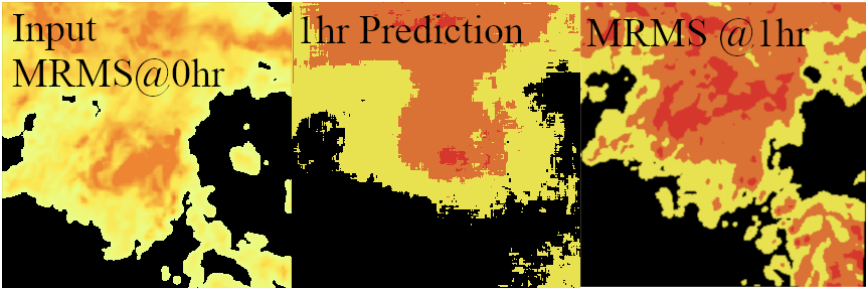
\includegraphics[keepaspectratio, scale=0.5]{fig/chapter1/Related_research_rainfall.png}
 \caption{1時間後先の降雨予測比較\cite{Related-Research2}}
 \label{R_r_r}
\end{figure}

\begin{figure}[H]
 \centering
 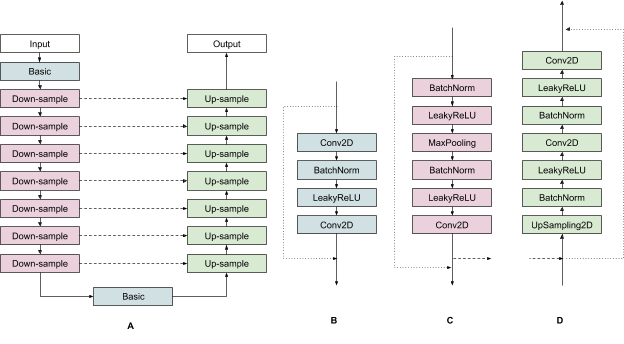
\includegraphics[keepaspectratio, scale=0.4]{fig/chapter1/rainfull_model.png}
 \caption{CNNモデルの詳細\cite{rainfull}}
 \label{rainfull_m}
\end{figure}
Jasonらの研究によるとこのCNNモデルを使用した1時間先の予測結果は既存のモデルoptical flow\cite{optical-flow}、persistence\cite{persistence}、HRRR nowcasting\cite{HRRR}と比較して精度が良くなるという研究結果がある。しかし、5時間先の予測の比較ではHRRRが良いという結果となった。\\
 結論としては 1 時間先という短時間予測においては CNN による画像から画像への予測変換モデルの有効性を示している。降水量の複雑な物理学をモデル化し、シミュレーションの時間がかかる手法をデータを入出力問題として扱うことで、1時間先の予測は良好であることを示している。しかしながら、HRRRと機械学習の両方のアプローチの組み合わせが問題として残る。\\
 Jasonらの研究を踏まえて降雨レーダー画像を使用した機械学習の問題ではCNNモデルがより良い精度を獲得できることがわかる。また、CNNを使用する理由の一つとして画像のデータの追加、交換が容易であることとしている。\\
 本研究では天候データである画像は地球の任意の場所で取得できるということもあり、特定の地域だけでなく任意の航路の欠航予測を行うこともできる拡張性に着目し、採用する。また、降雨レーダー画像と本研究で使用するデータセットの画像、図\ref{wind_data}、図\ref{wave_data}とは風、波と降雨のようにレイヤーが異なるだけなのでCNNモデルが有効だと考える。本研究の入力データは画像だが出力データは運航、欠航の2値分類のため出力結果を2値のクラス分類にする必要がある。
%そのため本研究でも画像入力の場合にCNNモデルを採用する。

%Jasonらの研究によってCNNが降雨レーダー画像に対して有効であると示されたために、本研究では天気予報の画像を入力データとして使用するため、学習モデルとしてCNNを用いる

%新しく「1.3 本研究の位置づけ」ぐらいの節を追加しよう。中身は、(1) 二値分類タスクとしての特徴(例えばレビュー分析のネガポジ判定と何が違うのか)、(2)天候予測との違い、(3)画像データや数値データとしての特徴(例えばImageNetとの違いは)、(4)時系列データとしての特徴、あたりを盛り込めるとベストです。(全部である必要はありません。少なくとも重要なポイントは示そう)
\section{本研究の位置づけ}
本研究は船舶の運航状況を欠航か運航か分類する二値分類タスクである。使用するデータとしては運航か欠航であるかの二値の教師データ、そこに付随する特徴量として数値データ(風速や波の高さ等)または画像データの2種類がある。これらの2種類のデータを分けて学習モデルに学習させ違いを比較することで、本研究の船舶での予測を行う際の最適なデータを検討する一助を目指し、さらに数値だけでの予測よりも精度向上を望めないか検討する。また、数日先までの予測を数値を使用した予測と画像を使用した予測を行った場合との違いを比較、考察を行い、数値と画像との精度評価を実施する。%どのようなデータが誤った予測しやすいのか明らかにしていく。

%画像を使用した機械学習としてImageNetが存在しているがImageNetでは様々な自然画像に対してそれぞれ1つずつラベルがついており、


%二値分類タスクでは他にレビュー分析のネガポジ判定がある。本研究では数値予測の他に画像での予測を行う、これは学習モデルに入力する情報が数値よりも画像の方がより多くの情報を持つのではないかと考えた結果である。

%\newpage

\section{論文の構成}
本論文は、以下の通りに構成されている。
\\
\\
\large{\textbf{第1章 はじめに}}\\
\ \ \ \ 本研究の背景と目的について述べる。\\
\large{\textbf{第2章 基礎概念}}\\
\ \ \ \ 提案手法に関することについて述べる。\\
\large{\textbf{第3章 提案手法}}\\
\ \ \ \ 機械学習の実装とデータ作成に関することについて述べる。\\
\large{\textbf{第4章 実験}}\\
\ \ \ \ 実験と考察について述べる。\\
\large{\textbf{第5章 今後の課題}}\\
\ \ \ \ 提案手法と検証に関する今後の課題を述べる。\\
\normalsize{}


%\section{Introduction}


% 基礎概念
\chapter{基礎概念}
\label{chap:concept}

\section{緒言}
船舶の運行状況予測をするにあたり、予測に使用した学習モデルや評価指標について述べる。

\section{CNN}
CNNとは畳み込みニューラルネットワークのことで畳み込み層やプーリング層などの層が積み重なったニューラルネットワークであり、
Y. LeCun\cite{Yann LeCun}らが最初に提唱した畳み込みニューラルネットワーク図\ref{lenet}が有名である。
画像を入力とした畳み込みニューラルネットワークの特徴的な層について説明する。
\begin{figure}[H]
 \centering
 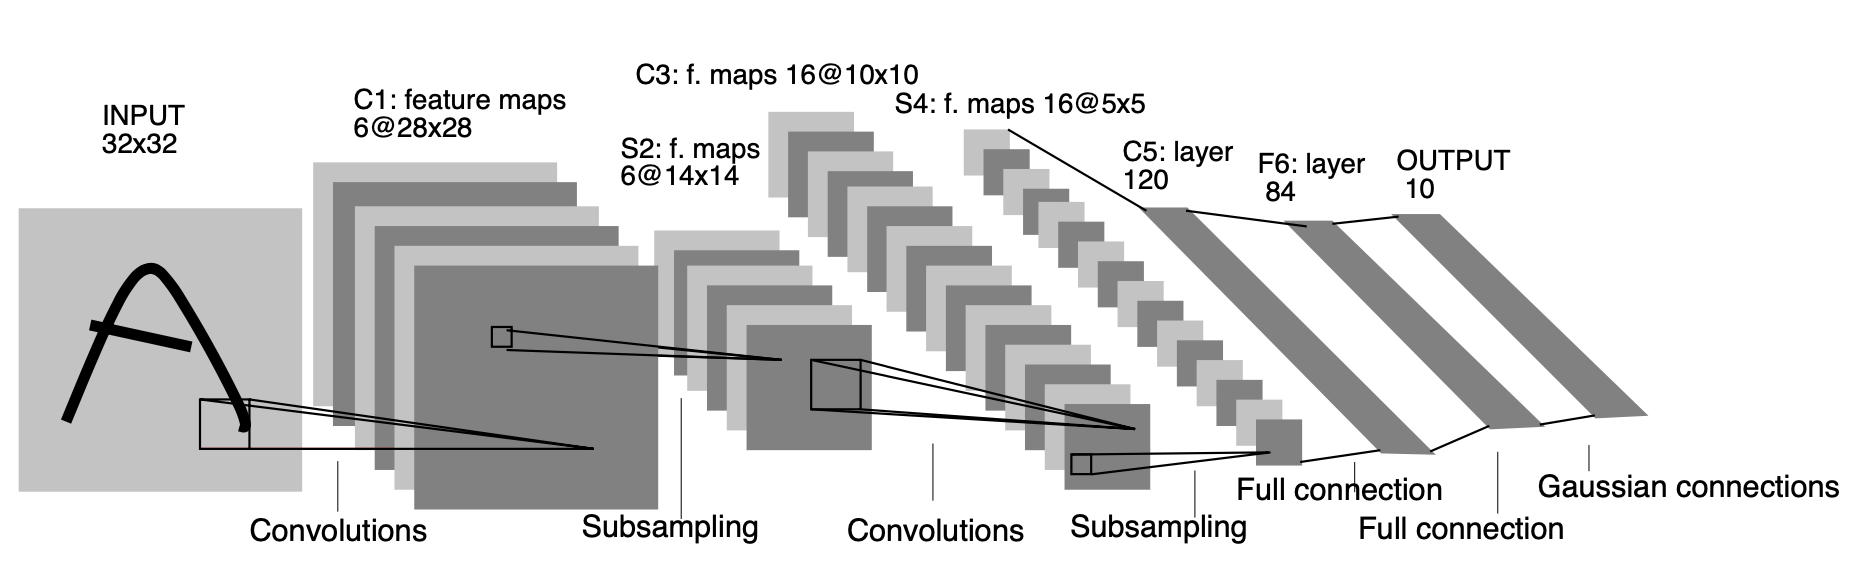
\includegraphics[keepaspectratio, scale=0.5]{fig/chapter2/Lenet-5.png}
 \caption{CNNの例\cite{Yann LeCun}}
 \label{lenet}
\end{figure}
\subsection{畳み込み層}
入力画像を畳み込み層に入力し画像から特徴を図\ref{tatami}にのように抽出する。
図\ref{tatami}では入力画像がカラー画像(RGB)の場合、入力に対してR、G、Bそれぞれのチャンネルに対して対応するフィルタを適用する。R、G、Bの入力に対してフィルタを重ね合わせ、合わせた部分の画素値に乗算を適用し合計値を算出、さらにR、G、Bの合計値により出力の画素値が決定し、その処理をスライドさせながら画像全体に対して行う。
\begin{figure}[H]
 \centering
 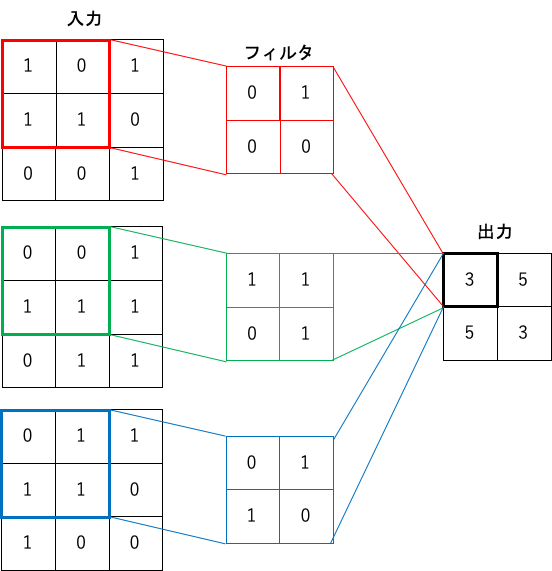
\includegraphics[keepaspectratio, scale=0.4]{fig/chapter2/tatamikomi.png}
 \caption{畳み込み層の出力例}
 \label{tatami}
\end{figure}

\subsection{プリーング層}
プーリング層とは入力画像内の局所的な情報を集めることである。とくにMax Poolingの図\ref{pooling}では入力に対して局所的な領域の最大値を出力する処理を行うことである。

\begin{figure}[H]
 \centering
 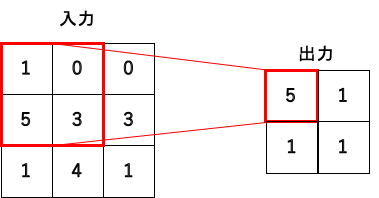
\includegraphics[keepaspectratio, scale=0.5]{fig/chapter2/pooling.png}
 \caption{プーリング層の出力例}
 \label{pooling}
\end{figure}


\section{LightGBM}
LightGBMとは決定木アルゴリズムをベースにした勾配ブースティングの機械学習フレームワークである。LightGBMの特徴として決定木、アンサンブル学習、勾配ブースティングなどがある。それぞれについて説明する。
\subsection{決定木}
LightGBMでは決定木を基にしたアルゴリズムを使用している。決定木とは図\ref{kettei}のように項目において閾値を決定し閾値により条件分岐させ木のように成長させて問題を解くアルゴリズムである。
\begin{figure}[H]
 \centering
 
\includegraphics[keepaspectratio, scale=0.6]{fig/chapter2/ketteigi.png}
 \caption{決定木の例}
 \label{kettei}
\end{figure}

\subsection{アンサンブル学習}
アンサンブル学習とは複数のモデルを学習させて1つの学習モデルを生み出す学種方法である。このようにすることで精度の低いモデルでも高精度な予測をすることができる。図\ref{ensemble}の例ではモデルの数を4つとしたときにそれぞれのモデルの予測結果の多数決をとることで最終的に100%の精度で予測することができる。
\begin{figure}[H]
 \centering
 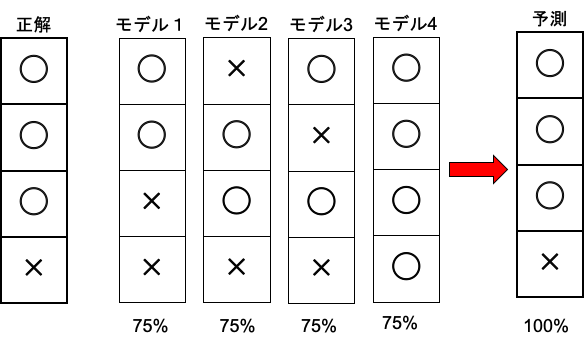
\includegraphics[keepaspectratio, scale=0.4]{fig/chapter2/ensemble.png}
 \caption{アンサンブルの例}
 \label{ensemble}
\end{figure}

\subsection{勾配ブースティング}
勾配ブースティングはアンサンブル学習の手法のひとつである。ブースティングとはデータセットの中から一部のデータを用いてモデルを学習し評価を行う。その後の別モデルで前のモデルで誤った予測をしたデータを学習し評価を行いさらに次のモデルでも同じことを行うことでデータの誤差の学習を行う。最後に各モデルの多数決を行いモデルを組み合わせる。

\section{windy.com}
本研究に使用したデータを取得してきたwebサイトである。このサイトは世界中の天気予報を可視化でき、リアルタイムの気象状況や気象値、数日先までの予報を閲覧することができる。レイヤー機能があり風速レイヤー、波高レイヤーや気温レイヤーなど様々なレイヤーを使用でき、レイヤーごとの特徴を視覚的に見ることができる\cite{windy}。

\section{安栄観光}
本研究に使用した教師データを取得してきたwebサイトである。このサイトでは主に石垣島から西表島への7つある航路の船舶運行状況を確認できる\cite{anei}。


\section{予測精度の評価指標}
本研究では上記で説明した学習モデルで入力を画像とする場合はCNNを採用し、数値を入力する場合はLightGBMを採用する。予報図(画像)、気象状況(数値)の比較を行うためそれぞれの予測精度を評価する必要がある。本研究の問題は二値分類問題であるので一般に正解率、適合率、再現率、F値を使用して評価をすることが多い。そのため本研究でもこれらの評価指標を用いて評価を行なう。%本節ではこれらの評価指標の説明を行う。

%\subsection{正解率}




%提案手法
\chapter{提案手法}
\label{chap:propose}

\section{データ作成}
本研究では八重山諸島の船舶航路を対象とし、安栄観光\cite{anei}と windy.com\cite{windy}というwebサイトからデータを取得し、機械学習を用いて欠航予測を行うことを目的とする。

\subsection{安栄観光、windy.comからデータの取得}
安栄観光\cite{anei}の運行状況のページから波照間島航路、西表島上原航路、鳩間島航路、西表島大原航路、小浜島航路、竹富島航路、黒島航路の7つの運行状況データを使用する。運行状況データにはそれぞれの航路別で出港時間毎に通常運行、欠航の情報がある。それぞれの航路は図\ref{aneikouro}となる。
\\ windy.com\cite{windy}では地球の任意の地点を選択し、天気予報などの様々な情報を確認することができる。八重山諸島航路は鳥瞰すると西表島と石垣島間を行き来する運行航路であることから、運行航路の北側、南側の2地点からデータを取得する。2地点の風速、最大風速、最大風速の風向、波高、波の向き、うねり、うねりの向き、うねりの間隔の数値データを対象とする。このデータは当日の7時から17時まで2時間間隔で取得し、当日から7日先までは0時から21時まで3時間間隔で確認することができ、当日から8日、9日、10日の3日間は3時から21時までの6時間間隔で確認できるため、以上のデータを取得する。また、気象データとしてWebページのスクリーンショットを当日から9日先までは7時から17時までの2時間間隔で取得し10日先に関しては7時から11時までを取得する。windy.com\cite{windy}ではレイヤーで風速、波高等の情報が分かれているため、その2種類のレイヤーで画像データとして取得する。
\\ 風速、波高データを取得する理由として、対象の航路の欠航判断基準\cite{stan}に風速、波高、視程等の項目があるため、参考にデータの取得範囲を風速、波高等に設定した。
\subsection{データセットの作成}
安栄観光\cite{anei}から得た運行状況データを教師データラベルとして、それ以外のデータを特徴量として機械学習にデータを適用するために前処理を行う。本研究では数値データと画像データを取得しているため、別々のデータセットとしてデータを作成していく。
前処理として取得した運行状況データは運行を0に、欠航を1の二値にエンコードする。画像データは画像を数値に変換するためにRGBの値にエンコードし$64\times64$のサイズにリサイズする。
\\ 例として1便の運行状況データを図\ref{anei_label}の赤枠を1サンプルの教師データとする。特徴量は運行状況データの時間帯周辺で取得された風速、波高等データを合わせたものを数値データのデータセットでは図\ref{value_data}のような例を1サンプルとする。画像データのデータセットでは風速、波高レイヤーでスクリーンショットを行った画像を特徴量とし図\ref{wind_data}、図\ref{wave_data}のように1サンプルとする。これらのサンプルデータの作成方法で数値、画像データを構築する。

\begin{figure}[H]
 \centering
 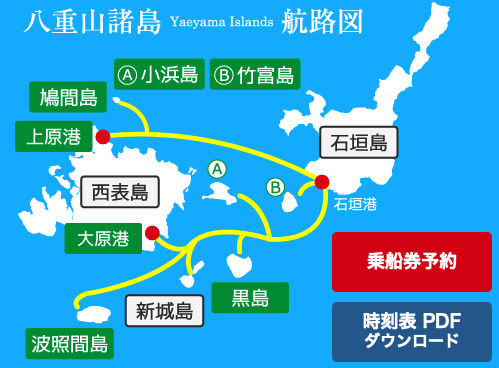
\includegraphics[keepaspectratio, scale=0.5]{fig/chapter3/aneikouro.png}
 \caption{安栄観光\cite{anei}の航路図}
 \label{aneikouro}
\end{figure}

\begin{figure}[H]
 \centering
 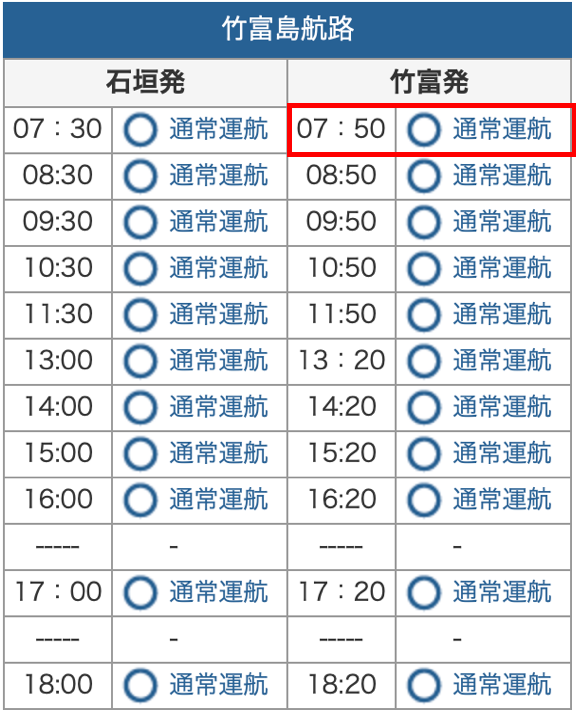
\includegraphics[keepaspectratio, scale=0.7]{fig/chapter3/anei_sample_data.png}
 \caption{安栄観光\cite{anei}の航路便運行状況}
 \label{anei_label}
\end{figure}

\begin{figure}[H]
 \centering
 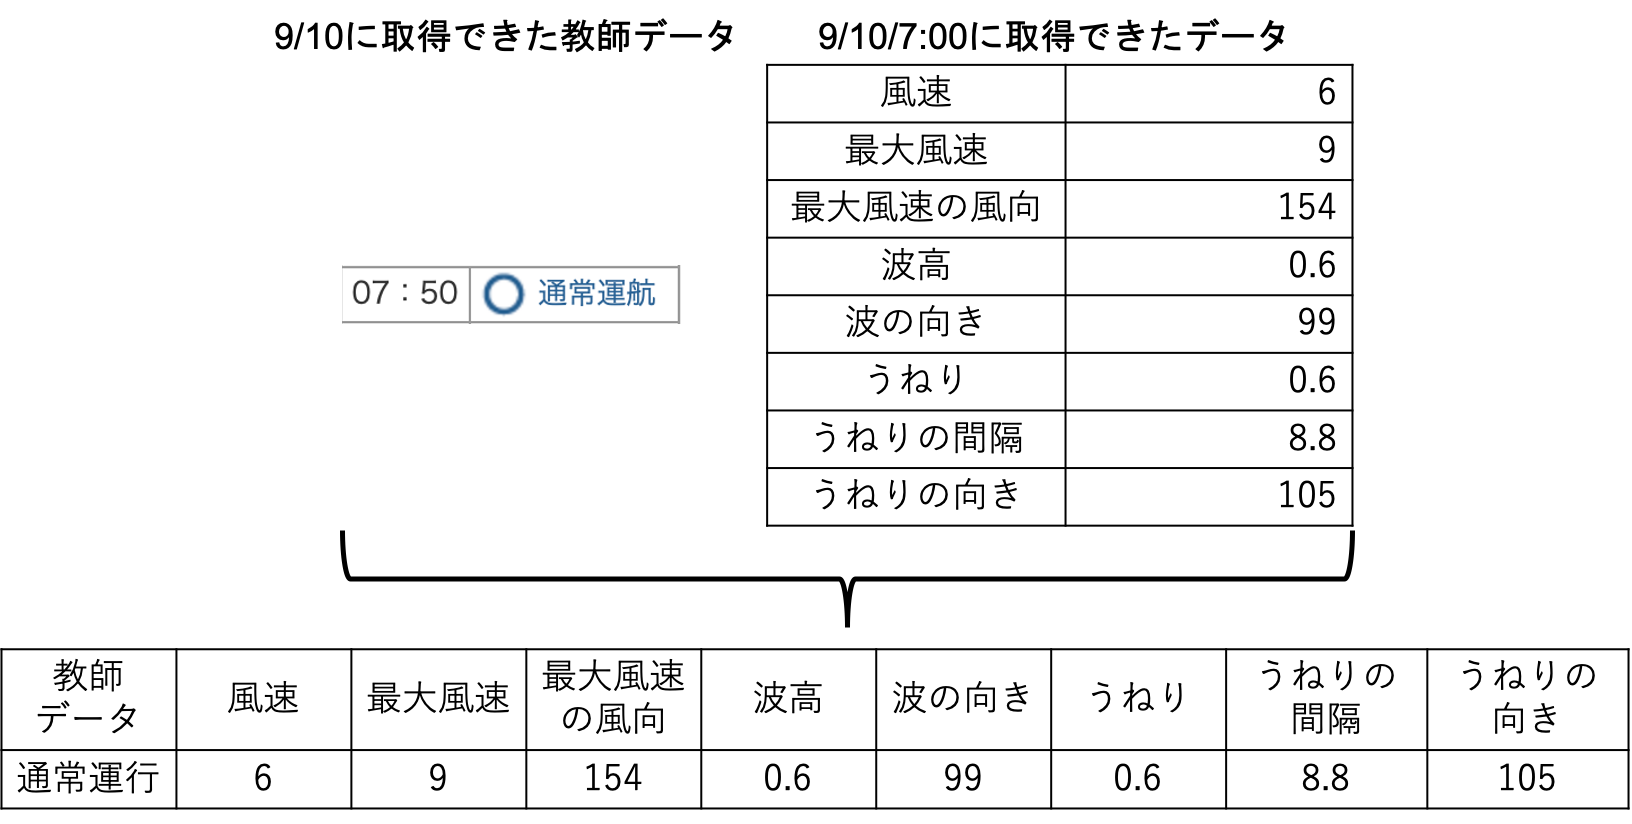
\includegraphics[keepaspectratio, scale=0.5]{fig/chapter3/value_dataset.png}
 \caption{数値データの作成例}
 \label{value_data}
\end{figure}



\begin{figure}[htbp]
 \begin{minipage}{0.5\hsize}
  \begin{center}
   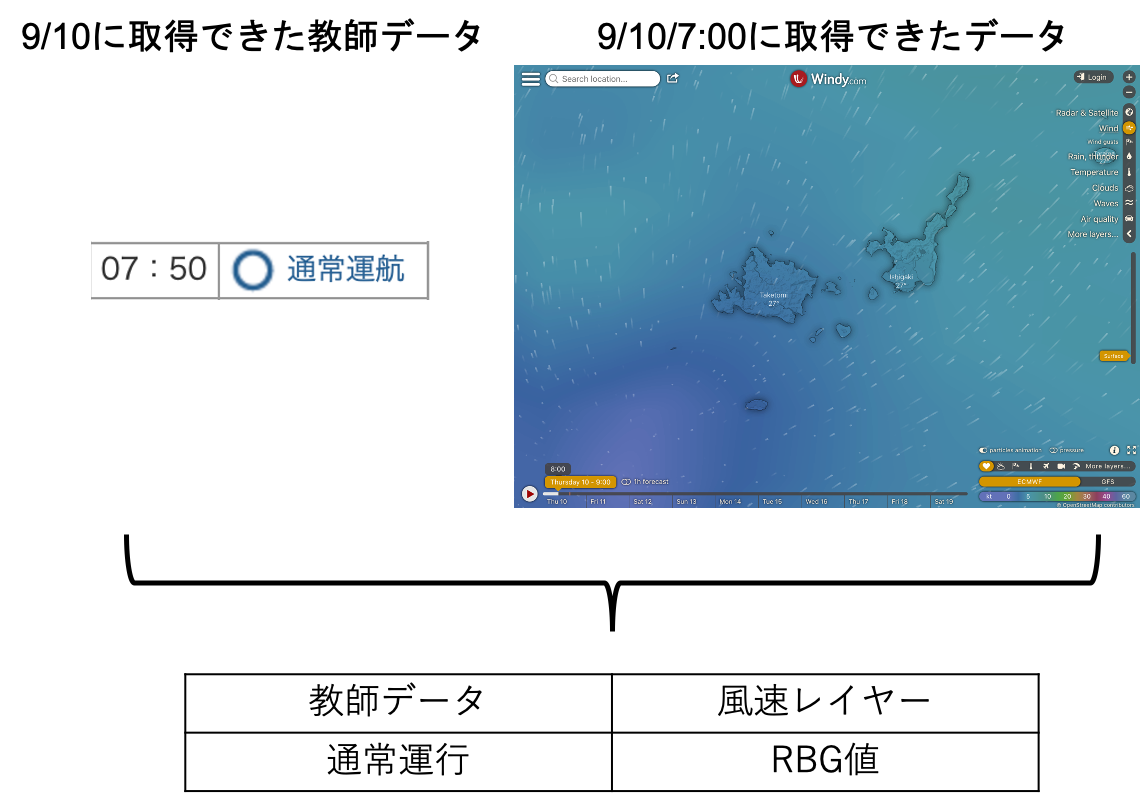
\includegraphics[keepaspectratio, scale=0.38]{fig/chapter3/wind_speed_data.png}
  \end{center}
  \caption{風速画像データの作成例}
  \label{wind_data}
 \end{minipage}
 \begin{minipage}{0.5\hsize}
  \begin{center}
  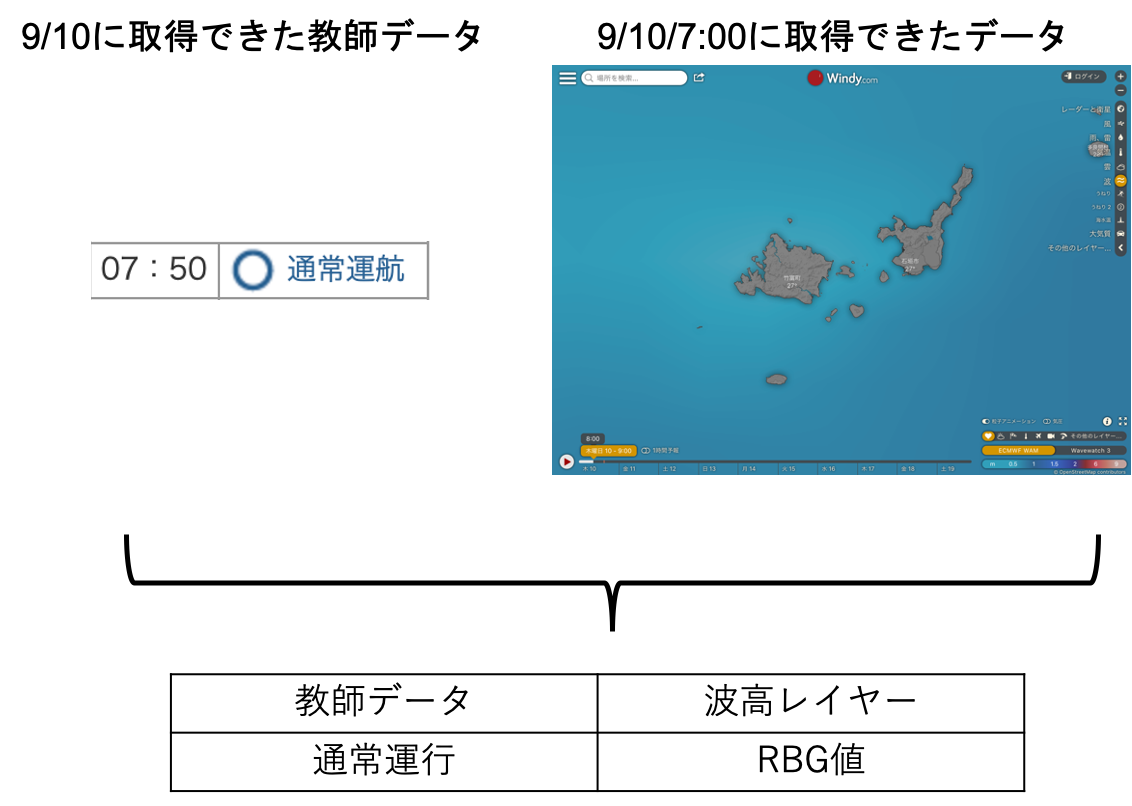
\includegraphics[keepaspectratio, scale=0.38]{fig/chapter3/wave_height_data.png}
  \end{center}
   \caption{波高画像データの作成例}
  \label{wave_data}
 \end{minipage}
\end{figure}

\section{運航状況の分類手法}
本研究では教師あり学習の分類問題として機械学習モデルを適用する。数値データセットではLightGBMを用い、画像データセットでは、CNNを使用する。
\subsection{学習モデル}
実験に使用したデータは大まかに2020年8月から2021年1月までの期間に取得できたものとなる。
学習モデルは航路に特化させるために航路ごとにデータセットを分けて学習を行うことで7航路あるうちのそれぞれに出発港が2つあるため$7\times2=14$個のモデルとなる。さらに、データを教師データの当日から$9=n$日前までの特徴量をスライドさせ当日のデータから当日の予測、n日前のデータからn日後の予測を行うためモデルを分けた。モデルを分けて作成したためモデルの総数は$14\times10=140$とし、数値データは図\ref{value_flow}となる。また画像データではさらに風速レイヤー、波高レイヤーで別々のデータセットのため$140\times2=280$個のモデルがあり、図\ref{img_flow}となる。

\begin{figure}[H]
 \centering
 
\includegraphics[keepaspectratio, scale=0.5]{fig/chapter3/value_flow.png}
 \caption{数値データの学習フロー}
 \label{value_flow}
\end{figure}

\begin{figure}[H]
 \centering
 
\includegraphics[keepaspectratio, scale=0.5]{fig/chapter3/img_flow.png}
 \caption{画像データの学習フロー}
 \label{img_flow}
\end{figure}







% 実験
\chapter{実験}
\label{chap:poordirection}

\section{実験結果}

\subsection{数値データによる結果}
数値データを用いた精度(正解率・適合率・再現率・F値)を表\ref{value_hatoma}、表\ref{value_kurosima}に示す。また、西表大原航路、小浜航路、竹富航路では欠航データが無く精度が100\%となったので省く、波照間航路や西表上原航路は表\ref{value_hatoma}のような傾向と似ている結果となったため省く。


\begin{table}[htbp]
  \begin{center}
    \begin{tabular}{c}
	%1
      \begin{minipage}{0.5\hsize}
        \begin{center}
          \caption{鳩間島航路-鳩間発}
          \begin{tabular}{|c|r|r|r|r|} \hline
   &正解率 & 適合率 & 再現率 & F値 \\ \hline
      当日&0.868 &0.933 &0.778 &0.848 \\ \hline
     1日前 & 0.816 & 0.875 & 0.737 & 0.800 \\ \hline
      2日前 & 0.816 & 0.929 & 0.684 & 0.788 \\ \hline
      3日前 & 0.649 & 0.636 & 0.737 & 0.683 \\ \hline 
      4日前 & 0.757 & 0.737 & 0.778 & 0.757 \\ \hline 
      5日前 & 0.639 & 0.667 & 0.556 & 0.667 \\ \hline 
      6日前 & 0.722 & 0.833 & 0.556 & 0.667 \\ \hline 
      7日前 & 0.583 & 0.562 & 0.529 & 0.545 \\ \hline 
      8日前 & 0.714 & 0.733 & 0.647 & 0.688 \\ \hline 
      9日前 & 0.629 & 0.625 & 0.588 & 0.606 \\ \hline 
          \end{tabular}
          \label{value_hatoma}
        \end{center}
      \end{minipage}
      %2
      \begin{minipage}{0.5\hsize}
        \begin{center}
          \caption{黒島航路-黒島発}
    \begin{tabular}{|c|r|r|r|r|} \hline
   &正解率 & 適合率 & 再現率 & F値 \\ \hline
      当日 & 1.000 & 1.000 & 1.000 & 1.000 \\ \hline
     1日前 & 0.987 & 0.000& 0.000 & 0.000 \\ \hline
      2日前 & 1.000 & 1.000 & 1.000 & 1.000 \\ \hline
      3日前 & 0.986 & 0.000 & 0.000 & 0.000 \\ \hline 
      4日前 & 1.000 & 0.000 & 0.000 & 0.000 \\ \hline 
      5日前 & 0.986 & 0.000 & 0.000 & 0.000 \\ \hline 
      6日前 & 0.986 & 0.000 & 0.000 & 0.000 \\ \hline 
      7日前 & 0.986 & 0.000 & 0.000 & 0.000 \\ \hline 
      8日前 & 1.000 & 1.000 & 1.000 & 1.000 \\ \hline 
      9日前 & 0.986 & 0.000 & 0.000 & 0.000 \\ \hline 
          \end{tabular}
           \label{value_kurosima}
        \end{center}
      \end{minipage}

    \end{tabular}
  \end{center}
\end{table}




\subsection{画像データによる結果}
画像データの波高レイヤーデータを用いた精度(正解率・適合率・再現率・F値)を表\ref{img_wave_hateruma}、表\ref{img_wave_hatoma}、表\ref{img_wave_taketomi}に示す。また、小浜島航路、黒島航路、西表大原航路は表\ref{img_wave_taketomi}と同様の結果が出力されたため省く、西表上原航路は表\ref{img_wave_hatoma}と傾向が似ているため省く。


\begin{table}[htbp]
  \begin{center}
    \begin{tabular}{c}
	%1
      \begin{minipage}{0.5\hsize}
        \begin{center}
          \caption{波高レイヤー(波照間航路-波照発)}
          \begin{tabular}{|c|r|r|r|r|} \hline
   &正解率 & 適合率 & 再現率 & F値 \\ \hline
      当日&0.796 &0.643 &0.643 &0.643 \\ \hline
     1日前 & 0.833 & 0.857 & 0.462 & 0.600 \\ \hline
      2日前 & 0.723 & 0.000 & 0.000 & 0.000 \\ \hline
      3日前 & 0.723 & 0.000 & 0.000 & 0.000 \\ \hline 
      4日前 & 0.756 & 0.000 & 0.000 & 0.000 \\ \hline 
      5日前 & 0.778 & 0.000 & 0.000 & 0.000 \\ \hline 
      6日前 & 0.773 & 0.000 & 0.000 & 0.000 \\ \hline 
      7日前 & 0.773 & 0.000 & 0.000 & 0.000 \\ \hline 
      8日前 & 0.773 & 0.000 & 0.000 & 0.000 \\ \hline 
      9日前 & 0.767 & 0.000 & 0.000 & 0.000 \\ \hline 
          \end{tabular}
          \label{img_wave_hateruma}
        \end{center}
      \end{minipage}
      %2
      \begin{minipage}{0.5\hsize}
        \begin{center}
          \caption{波高レイヤー(鳩間島航路-鳩間発)}
    \begin{tabular}{|c|r|r|r|r|} \hline
   &正解率 & 適合率 & 再現率 & F値 \\ \hline
      当日 & 0.882 & 0.929 & 0.812 & 0.867 \\ \hline
     1日前 & 0.818 & 0.917 & 0.688 & 0.786 \\ \hline
      2日前 & 0.727 & 0.818 & 0.562 & 0.667 \\ \hline
      3日前 & 0.562 & 0.545 & 0.400 & 0.462 \\ \hline 
      4日前 & 0.594 & 0.538 & 0.500 & 0.519 \\ \hline 
      5日前 & 0.645 & 0.615 & 0.571 & 0.593 \\ \hline 
      6日前 & 0.613 & 0.600 & 0.429 & 0.500 \\ \hline 
      7日前 & 0.581 & 0.545 & 0.429 & 0.480 \\ \hline 
      8日前 & 0.700 & 0.647 & 0.786 & 0.710 \\ \hline 
      9日前 & 0.667 & 0.667 & 0.571 & 0.615 \\ \hline 
          \end{tabular}
          \label{img_wave_hatoma}
        \end{center}
      \end{minipage}

    \end{tabular}
  \end{center}
\end{table}

\begin{table}[H]
  \begin{center}
    \caption{波高レイヤー(竹富航路-竹富発)}
    \begin{tabular}{|c|r|r|r|r|} \hline
   &正解率 & 適合率 & 再現率 & F値 \\ \hline
      当日 & 0.990 & 0.000 & 0.000 & 0.000 \\ \hline
     1日前 & 0.979 & 0.000 & 0.000 & 0.000 \\ \hline
      2日前 & 0.974 & 0.000 & 0.000 & 0.000 \\ \hline
      3日前 & 0.973 & 0.000 & 0.000 & 0.000 \\ \hline 
      4日前 & 0.972 & 0.000 & 0.000 & 0.000 \\ \hline 
      5日前 & 0.972 & 0.000 & 0.000 & 0.000 \\ \hline 
      6日前 & 0.977 & 0.000 & 0.000 & 0.000 \\ \hline 
      7日前 & 0.989 & 0.000 & 0.000 & 0.000 \\ \hline 
      8日前 & 0.994 & 0.000 & 0.000 & 0.000 \\ \hline 
      9日前 & 0.994 & 0.000 & 0.000 & 0.000 \\ \hline 
    \end{tabular}    
    \label{img_wave_taketomi}
  \end{center}
\end{table}

画像データの風速レイヤーデータを用いた精度(正解率・適合率・再現率・F値)を表\ref{img_wind_hateruma}、表\ref{img_wind_iriue}、表\ref{img_wind_taketomi}に示す。また、小浜島航路、黒島航路、西表大原航路は表\ref{img_wind_iriue}と同様の結果が出力されたため省く、鳩間島航路は表\ref{img_wind_iriue}と傾向が似ているため省く。

\begin{table}[htbp]
  \begin{center}
    \begin{tabular}{c}
	%1
      \begin{minipage}{0.5\hsize}
        \begin{center}
          \caption{風速レイヤー(波照間航路-波照発)}
          \begin{tabular}{|c|r|r|r|r|} \hline
   &正解率 & 適合率 & 再現率 & F値 \\ \hline
      当日&0.776 &0.579 &0.786 &0.667 \\ \hline
     1日前 & 0.812 & 0.750 & 0.462 & 0.571 \\ \hline
      2日前 & 0.729 & 0.000 & 0.000 & 0.000 \\ \hline
      3日前 & 0.723 & 0.000 & 0.000 & 0.000 \\ \hline 
      4日前 & 0.756 & 0.000 & 0.000 & 0.000 \\ \hline 
      5日前 & 0.778 & 0.000 & 0.000 & 0.000 \\ \hline 
      6日前 & 0.773 & 0.000 & 0.000 & 0.000 \\ \hline 
      7日前 & 0.773 & 0.000 & 0.000 & 0.000 \\ \hline 
      8日前 & 0.750 & 0.000 & 0.000 & 0.000 \\ \hline 
      9日前 & 0.767 & 0.000 & 0.000 & 0.000 \\ \hline 
          \end{tabular}
          \label{img_wind_hateruma}
        \end{center}
      \end{minipage}
      %2
      \begin{minipage}{0.5\hsize}
        \begin{center}
          \caption{風速レイヤー(西表上原航路-西表上原発)}
    \begin{tabular}{|c|r|r|r|r|} \hline
   &正解率 & 適合率 & 再現率 & F値 \\ \hline
      当日 & 0.846 & 0.863 & 0.786 & 0.822 \\ \hline
     1日前 & 0.803 & 0.971 & 0.589 & 0.733 \\ \hline
      2日前 & 0.708 & 0.769 & 0.536 & 0.632 \\ \hline
      3日前 & 0.619 & 0.610 & 0.463 & 0.526 \\ \hline 
      4日前 & 0.696 & 0.684 & 0.531 & 0.598 \\ \hline 
      5日前 & 0.649 & 0.610 & 0.510 & 0.556 \\ \hline 
      6日前 & 0.598 & 0.562 & 0.367 & 0.444 \\ \hline 
      7日前 & 0.527 & 0.429 & 0.180 & 0.254 \\ \hline 
      8日前 & 0.709 & 0.630 & 0.902 & 0.742 \\ \hline 
      9日前 & 0.697 & 0.638 & 0.755 & 0.692 \\ \hline 
          \end{tabular}
          \label{img_wind_iriue}
        \end{center}
      \end{minipage}

    \end{tabular}
  \end{center}
\end{table}

\begin{table}[H]
  \begin{center}
    \caption{風速レイヤー(竹富航路-竹富発)}
    \begin{tabular}{|c|r|r|r|r|} \hline
   &正解率 & 適合率 & 再現率 & F値 \\ \hline
      当日 & 0.990 & 0.000 & 0.000 & 0.000 \\ \hline
     1日前 & 0.979 & 0.000 & 0.000 & 0.000 \\ \hline
      2日前 & 0.974 & 0.000 & 0.000 & 0.000 \\ \hline
      3日前 & 0.973 & 0.000 & 0.000 & 0.000 \\ \hline 
      4日前 & 0.978 & 0.000 & 0.000 & 0.000 \\ \hline 
      5日前 & 0.989 & 1.000 & 0.600 & 0.750 \\ \hline 
      6日前 & 0.978 & 0.000 & 0.000 & 0.000 \\ \hline 
      7日前 & 0.989 & 0.000 & 0.000 & 0.000 \\ \hline 
      8日前 & 0.994 & 0.000 & 0.000 & 0.000 \\ \hline 
      9日前 & 0.994 & 0.000 & 0.000 & 0.000 \\ \hline 
    \end{tabular}
    \label{img_wind_taketomi}
  \end{center}
\end{table}


\section{考察}

\subsection{数値データの考察}

表\ref{value_hatoma}の鳩間島航路-鳩間発1日前モデルにおけるテストデータの予測結果別に色分けをした散布図が図\ref{hatoma_1_scatter_pred}になる。この図を見ると特徴量wave\_heightの箇所で明確な色分けがおこなわれているのが確認でき、教師ラベルとの強い関係性を見ることができる。この結果から1日前モデルがwave\_heightを重要な特徴量として処理していると考えられる。
そこで、9日前モデルの散布図\ref{hatoma_9_scatter_pred}を見ると各特徴量と教師データとの結びつきが弱くなっていることが確認できる。そのため9日前モデルでは表\ref{value_hatoma}で示されているように予測精度が悪くなっていることが説明できる。これはデータセット作成する際、特徴量と教師ラベルを9日間ずらして作成しているため、1日前と比較して特徴量が運航や欠航を説明するための情報が減少していると考えられる。

\begin{figure}[H]
 \centering
 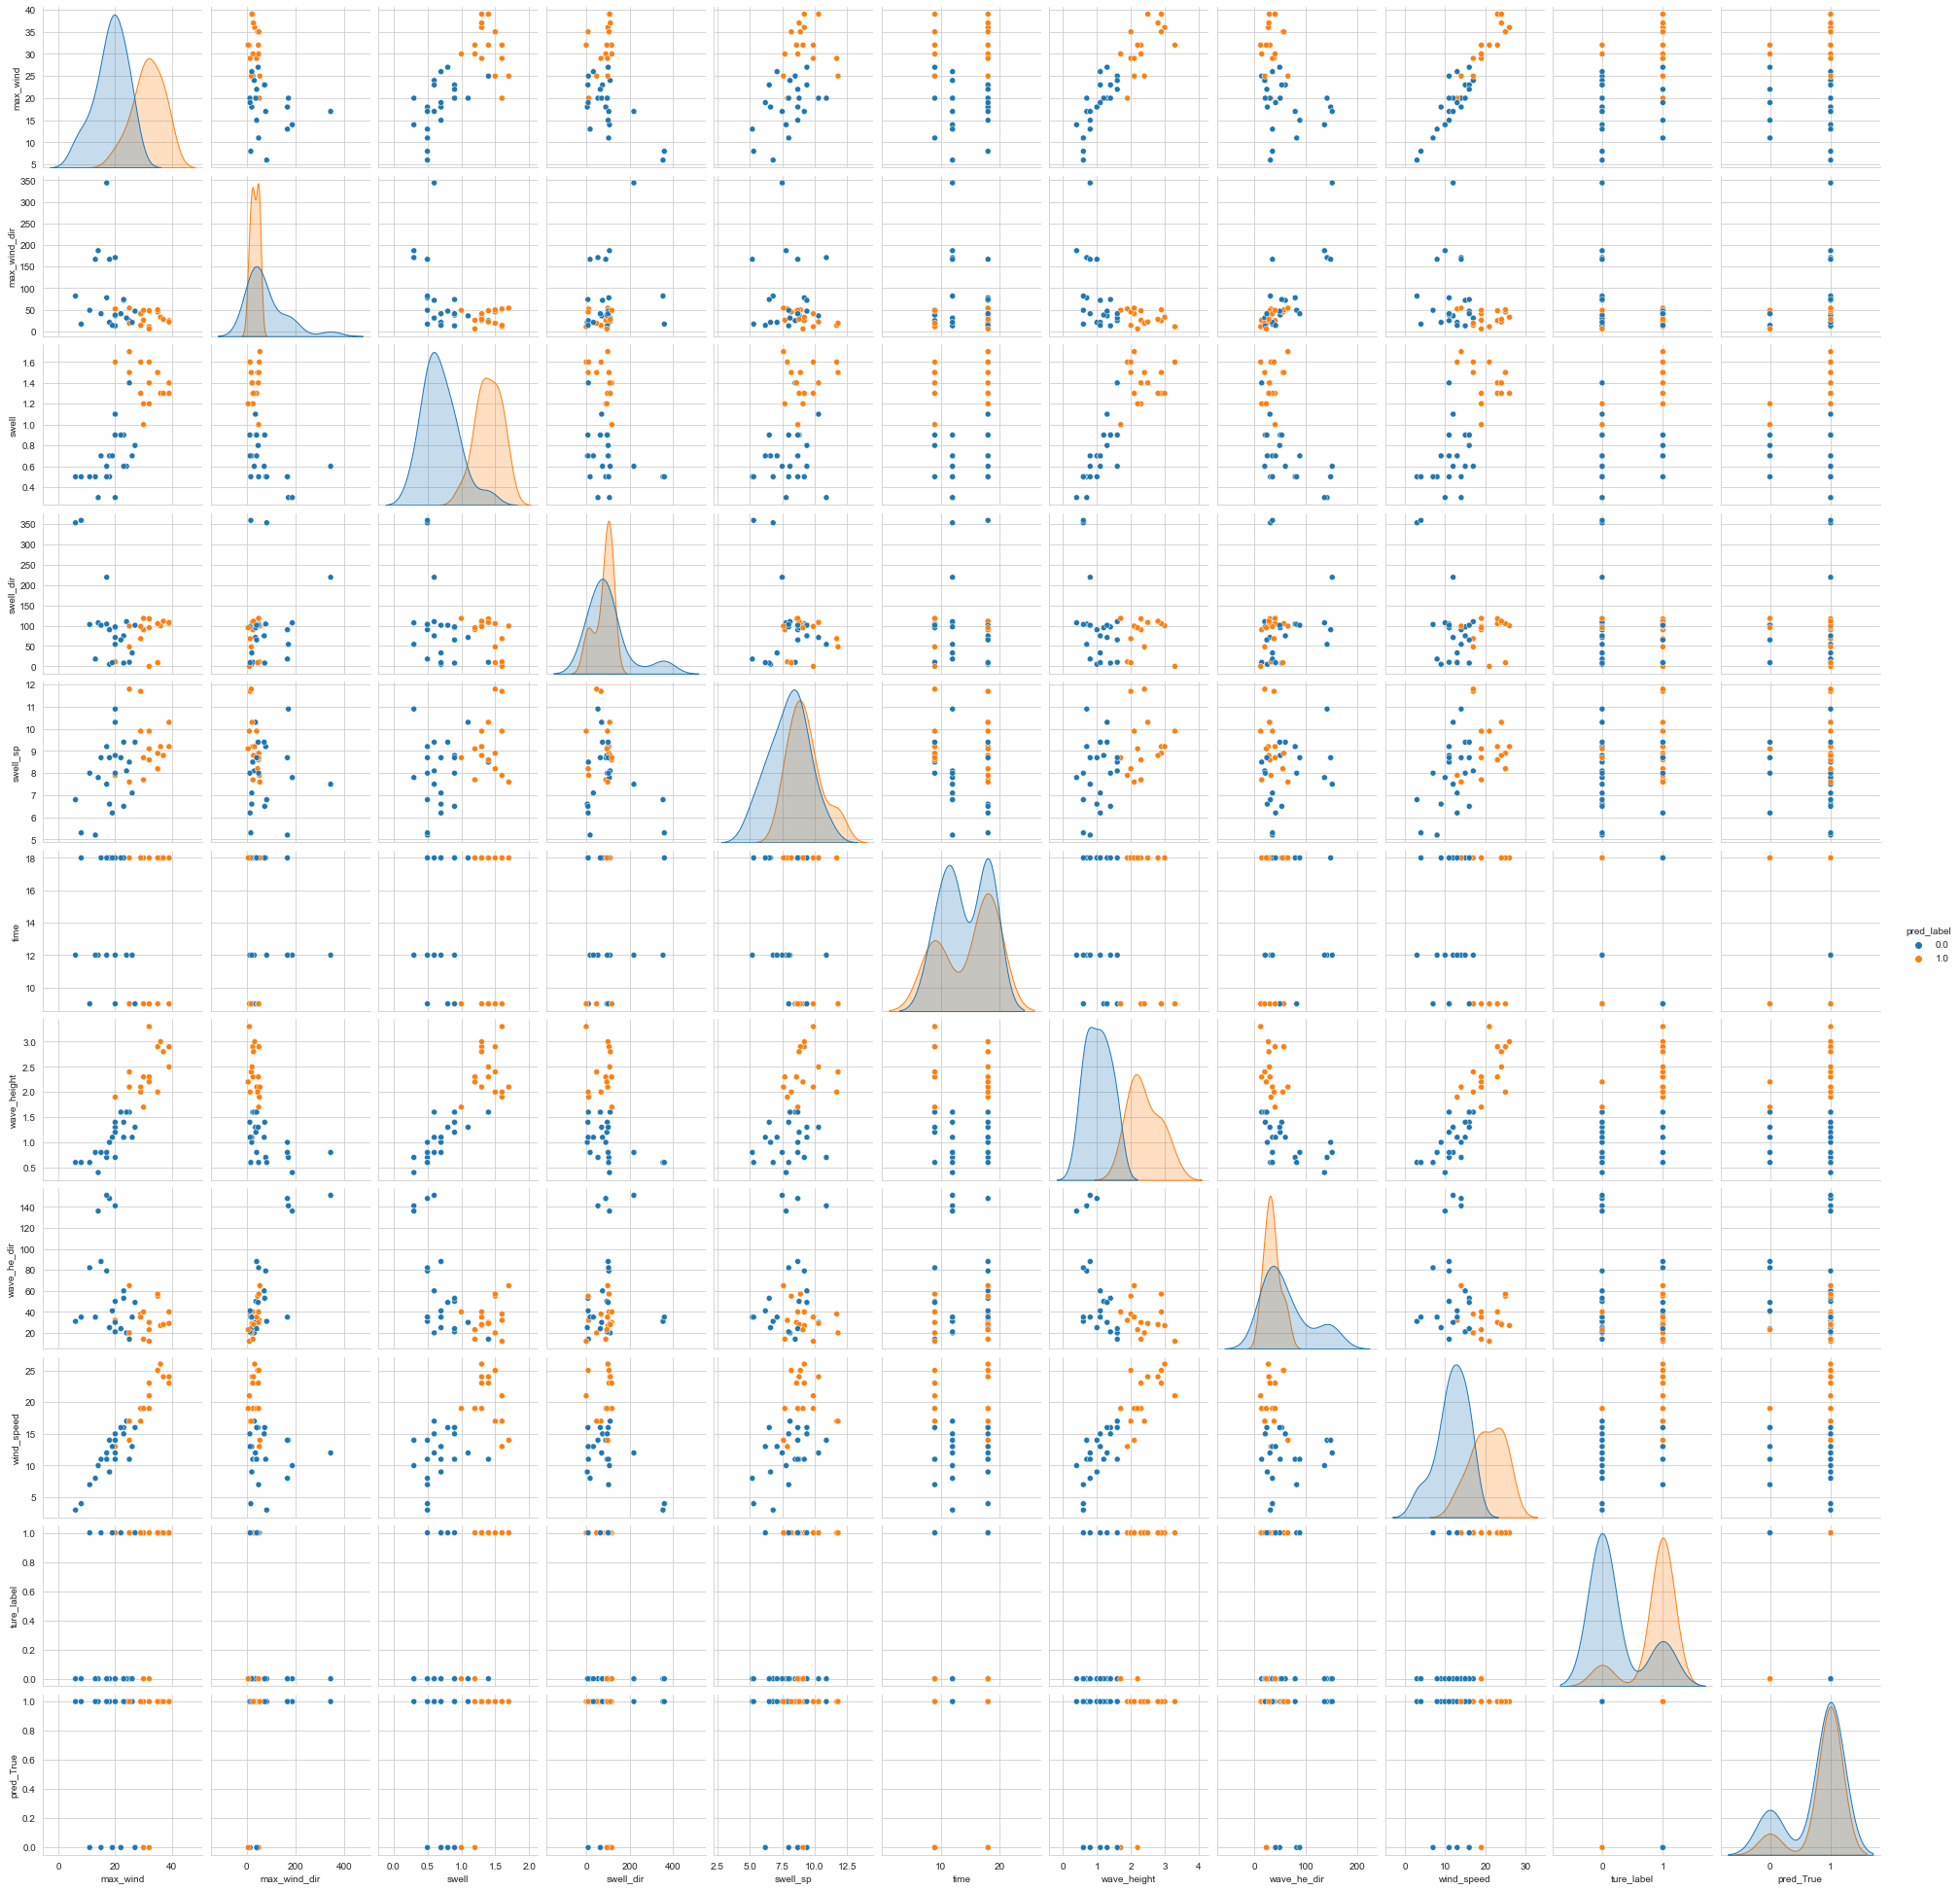
\includegraphics[keepaspectratio, scale=0.25]{fig/chapter4/hatoma_1_pred.png}
 \caption{鳩間島航路1日前モデルの予測ラベル}
 \label{hatoma_1_scatter_pred}
\end{figure}

\begin{figure}[H]
 \centering
 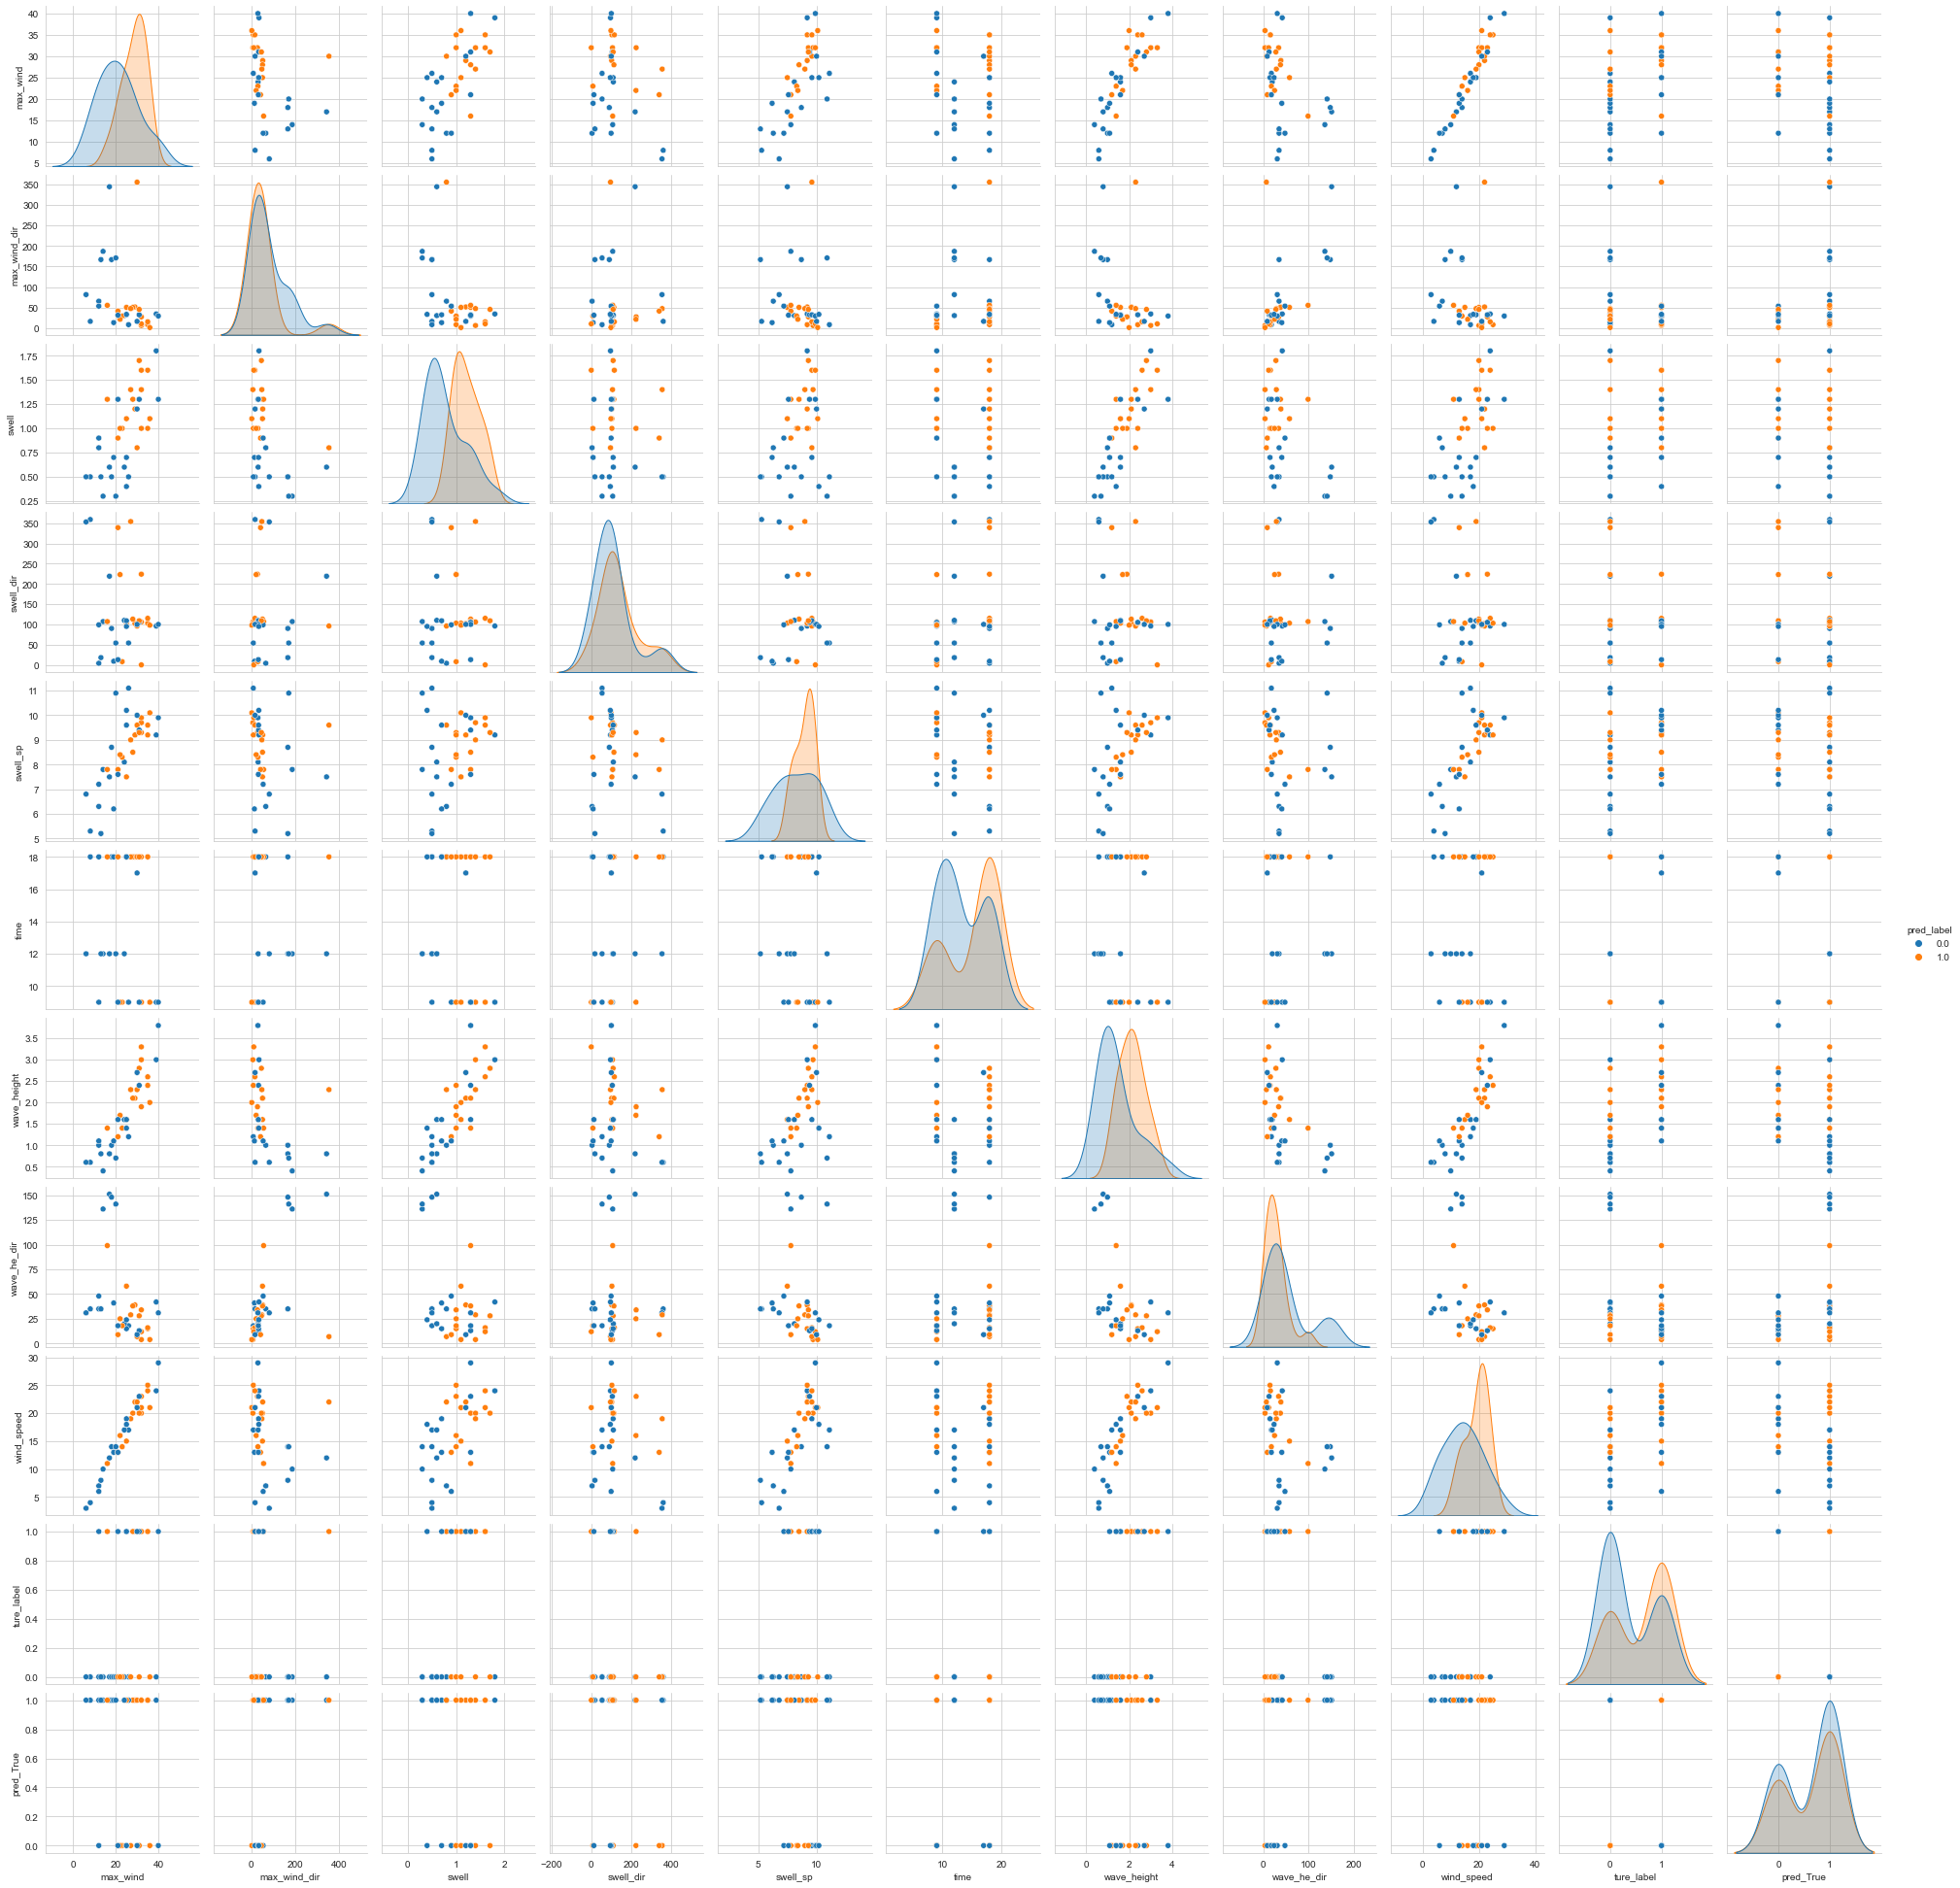
\includegraphics[keepaspectratio, scale=0.25]{fig/chapter4/hatoma_9_pred.png}
 \caption{鳩間島航路9日前モデルの予測ラベル}
 \label{hatoma_9_scatter_pred}
\end{figure}

表\ref{value_kurosima}から黒島航路-黒島発当日モデルの結果では全ての評価指標において1.000を獲得しており精度がとても良いことがわかる。当日モデルのテストデータの予測結果別に色分けをした散布図\ref{kurosima_0_scatter_pred}を確認すると、テストデータにある唯一の欠航データの特徴をしっかり捉えて予測できたことが確認できる。しかし、表\ref{value_kurosima}の1日前モデルの評価結果では正解率0.987とよく見えるがF値が0.000となっており欠航データに対する予測が全くできていないことが見て取れる。散布図\ref{kurosima_1_scatter_pred}を見てもわかるように全て運航すると予測されている。そこで、1日前モデルで用いたテストデータの教師ラベルを真値で色分けした散布図\ref{kurosima_1_scatter_ture}を見ると欠航データであるオレンジ点が青色の運航データの集団の中に分布していることが確認できる。このことからデータセットの教師データを1日ずらしたモデルの1日前モデルではデータセットをずらすことで欠航という情報を維持できず、運航のデータと変わらないデータになっていることが考えられる。


\begin{figure}[H]
 \centering
 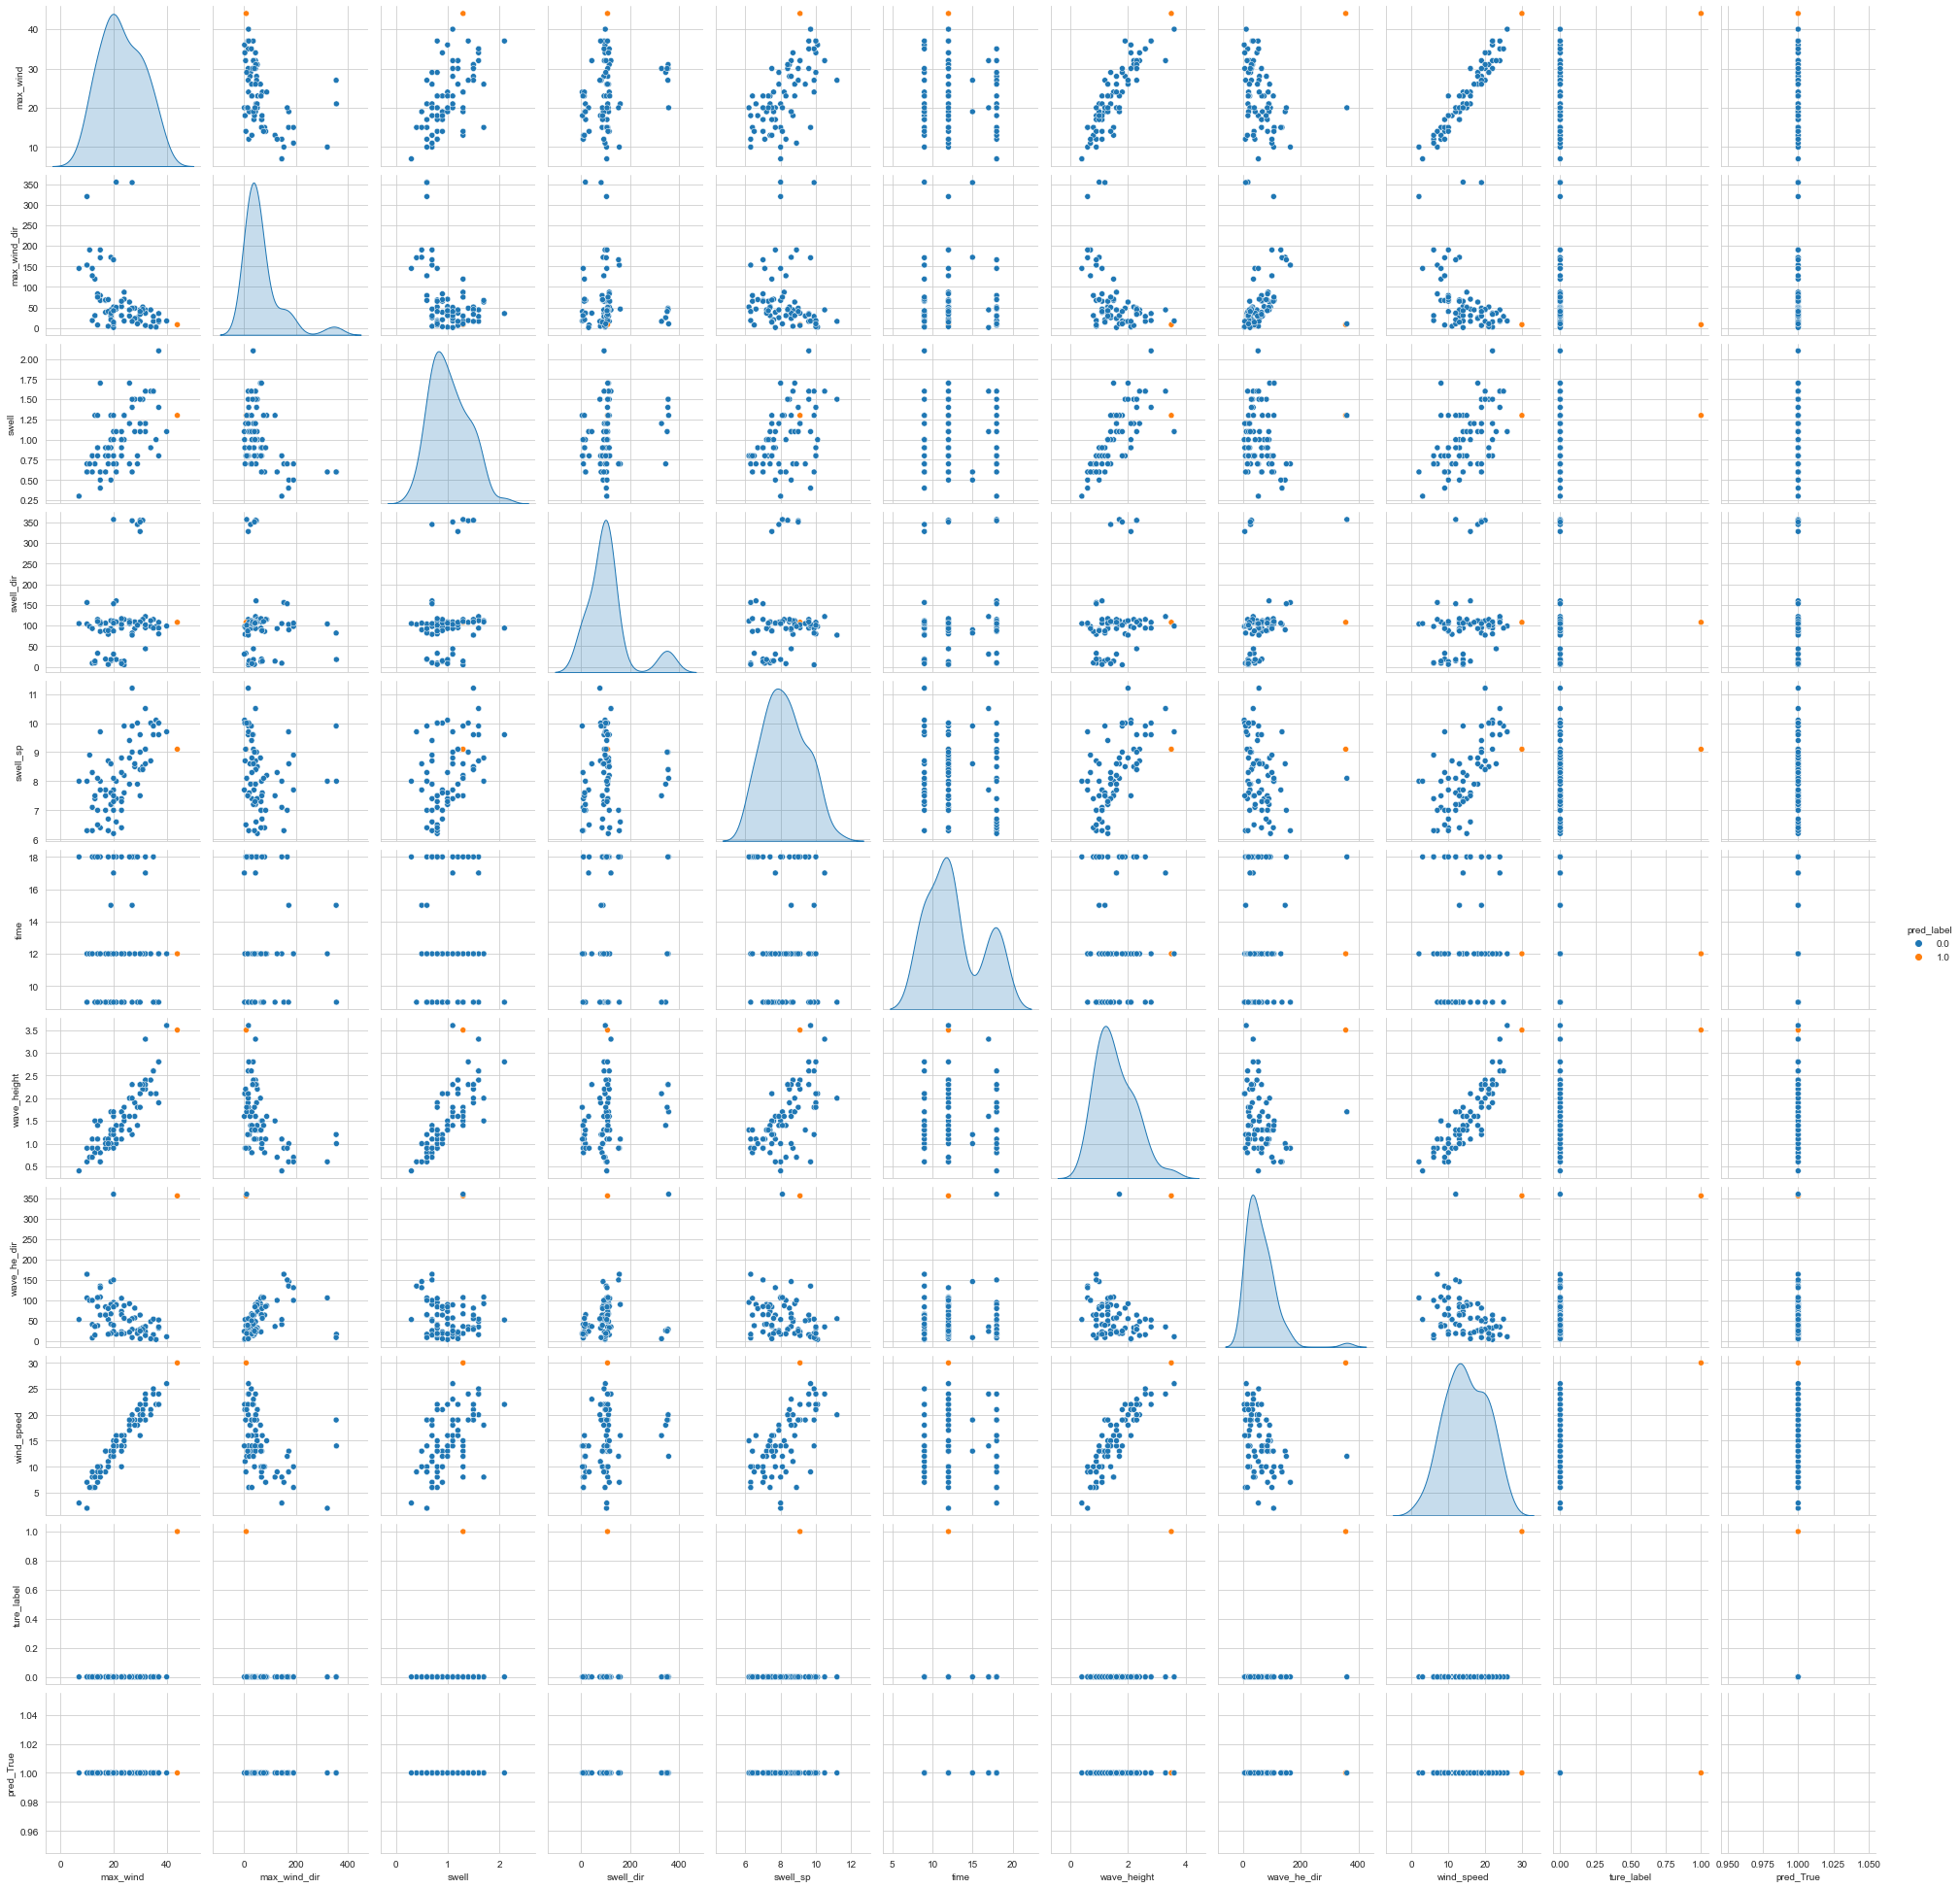
\includegraphics[keepaspectratio, scale=0.25]{fig/chapter4/kurosima_0_pred.png}
 \caption{黒島航路当日モデルの予測ラベル別}
 \label{kurosima_0_scatter_pred}
\end{figure}

\begin{figure}[H]
 \centering
 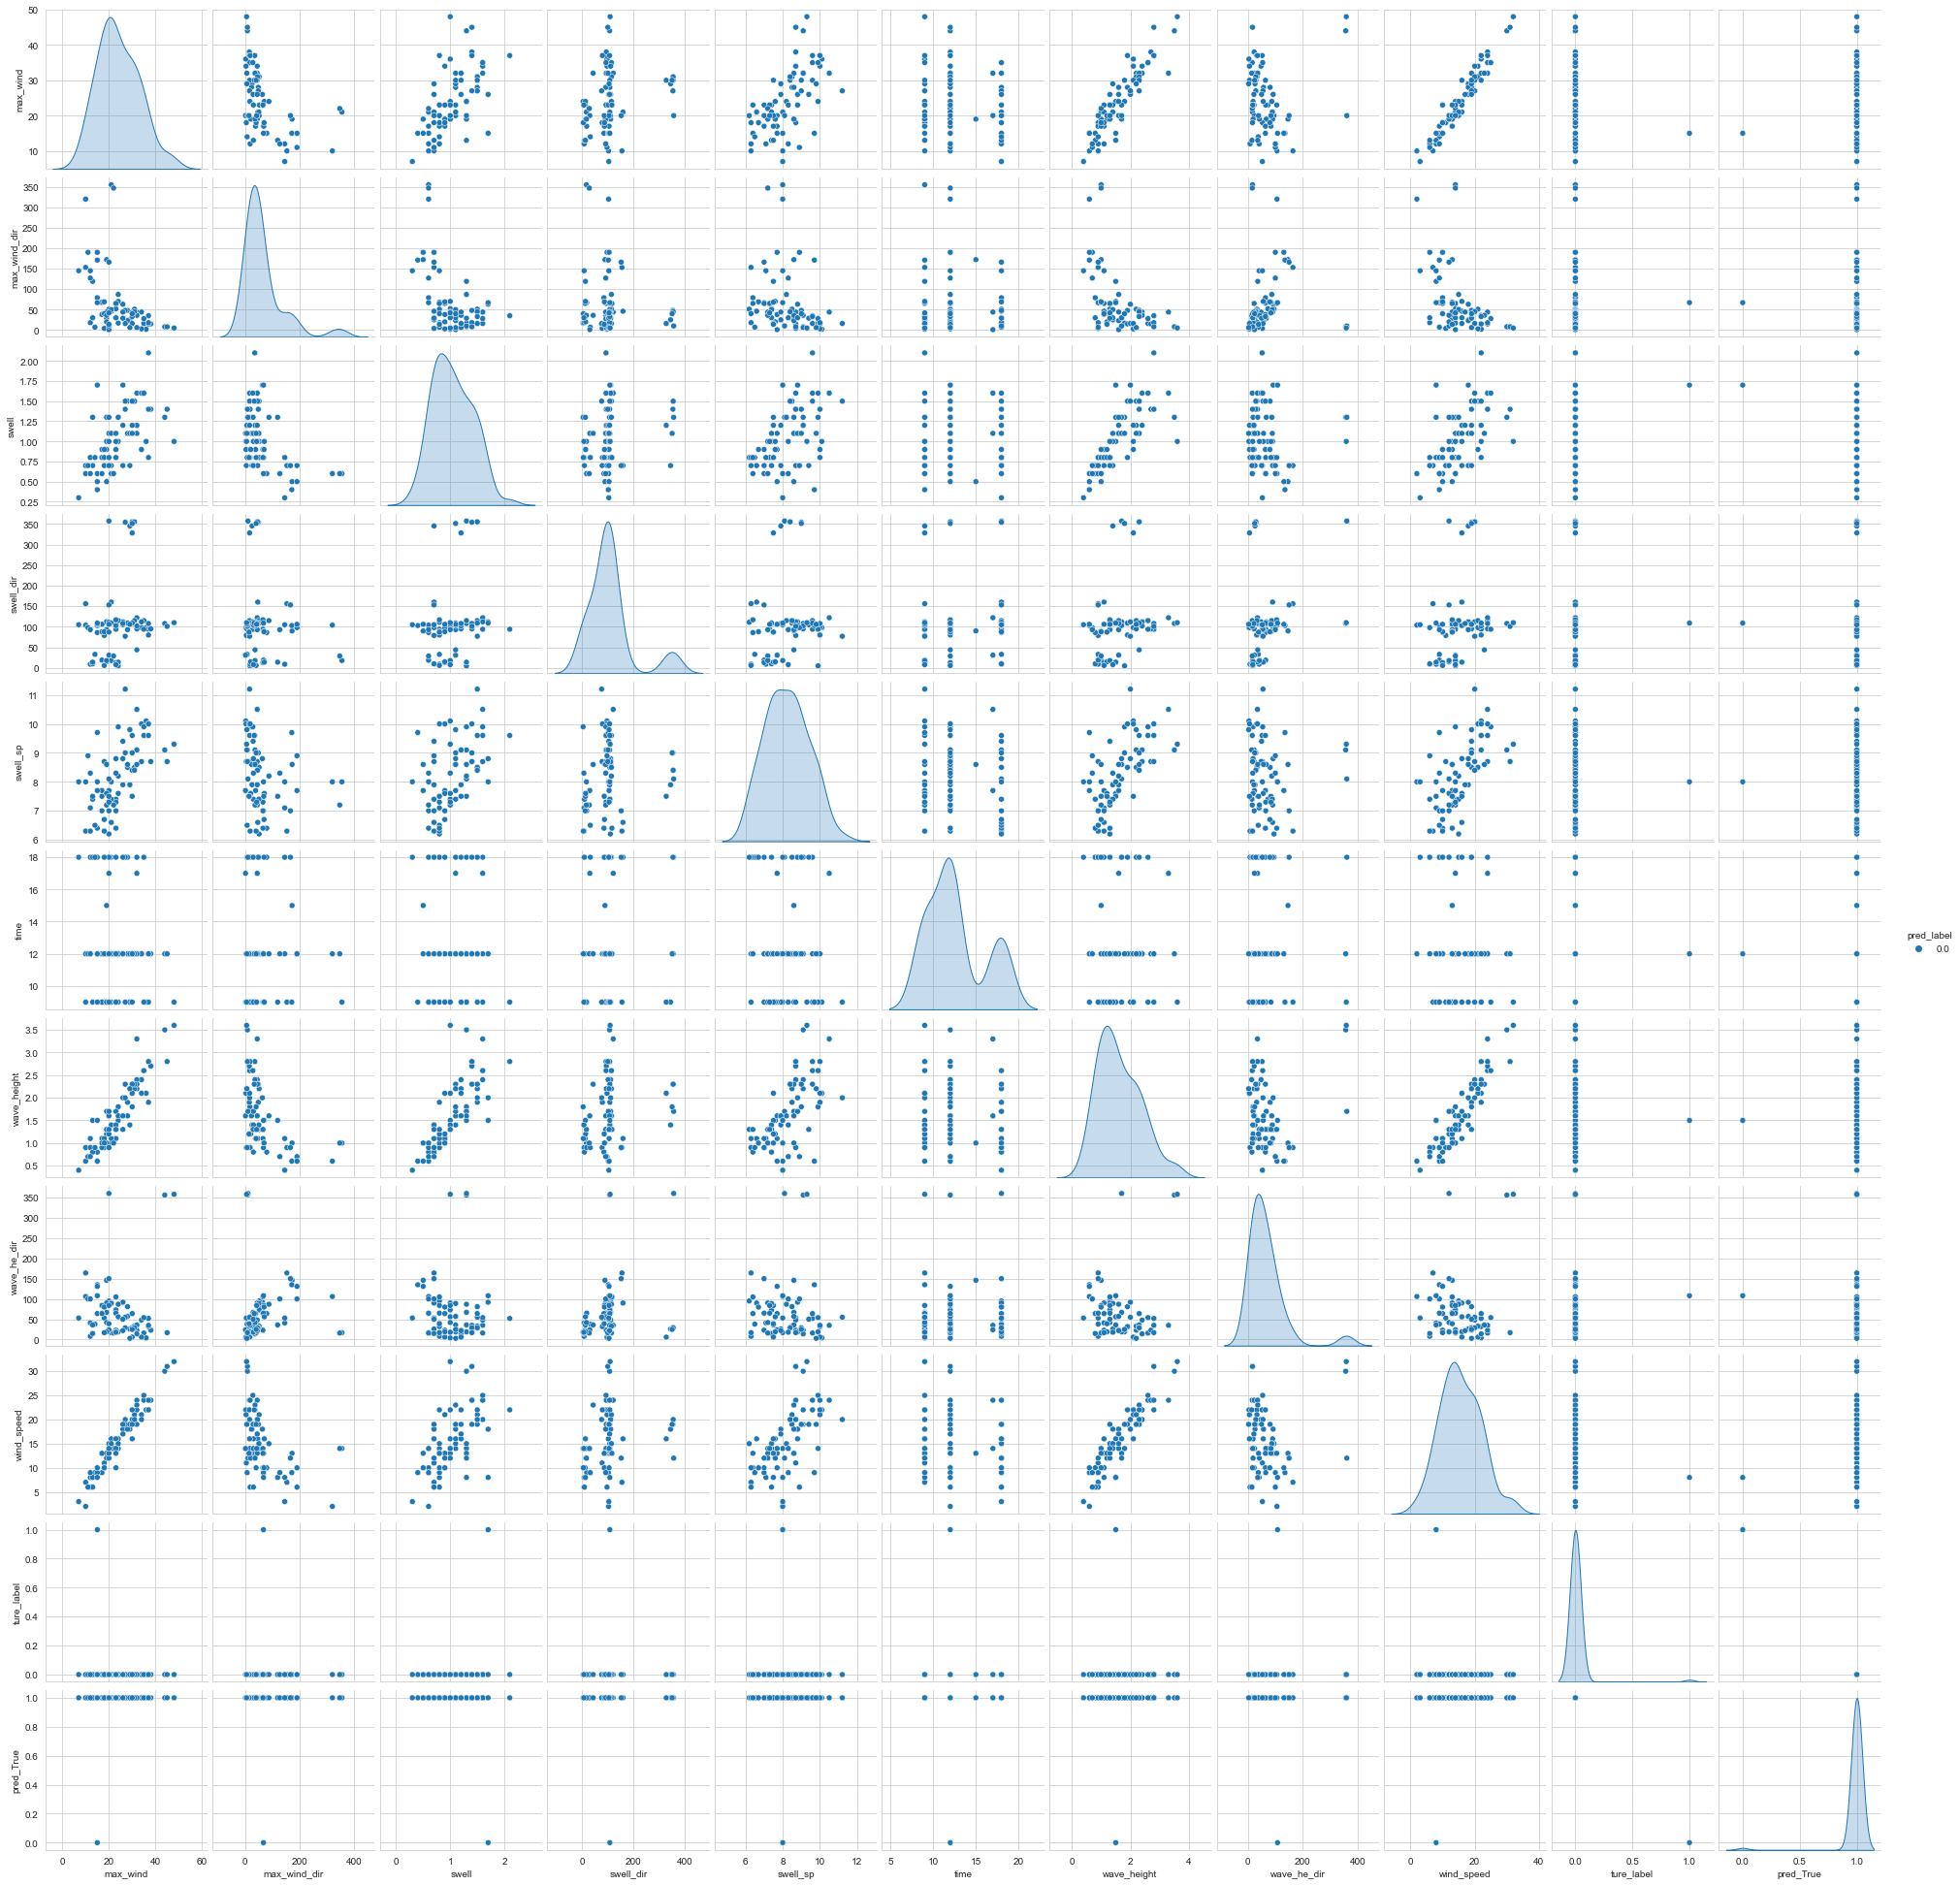
\includegraphics[keepaspectratio, scale=0.25]{fig/chapter4/kurosima_1_pred.png}
 \caption{黒島航路1日前モデルの予測ラベル別}
 \label{kurosima_1_scatter_pred}
\end{figure}

\begin{figure}[H]
 \centering
 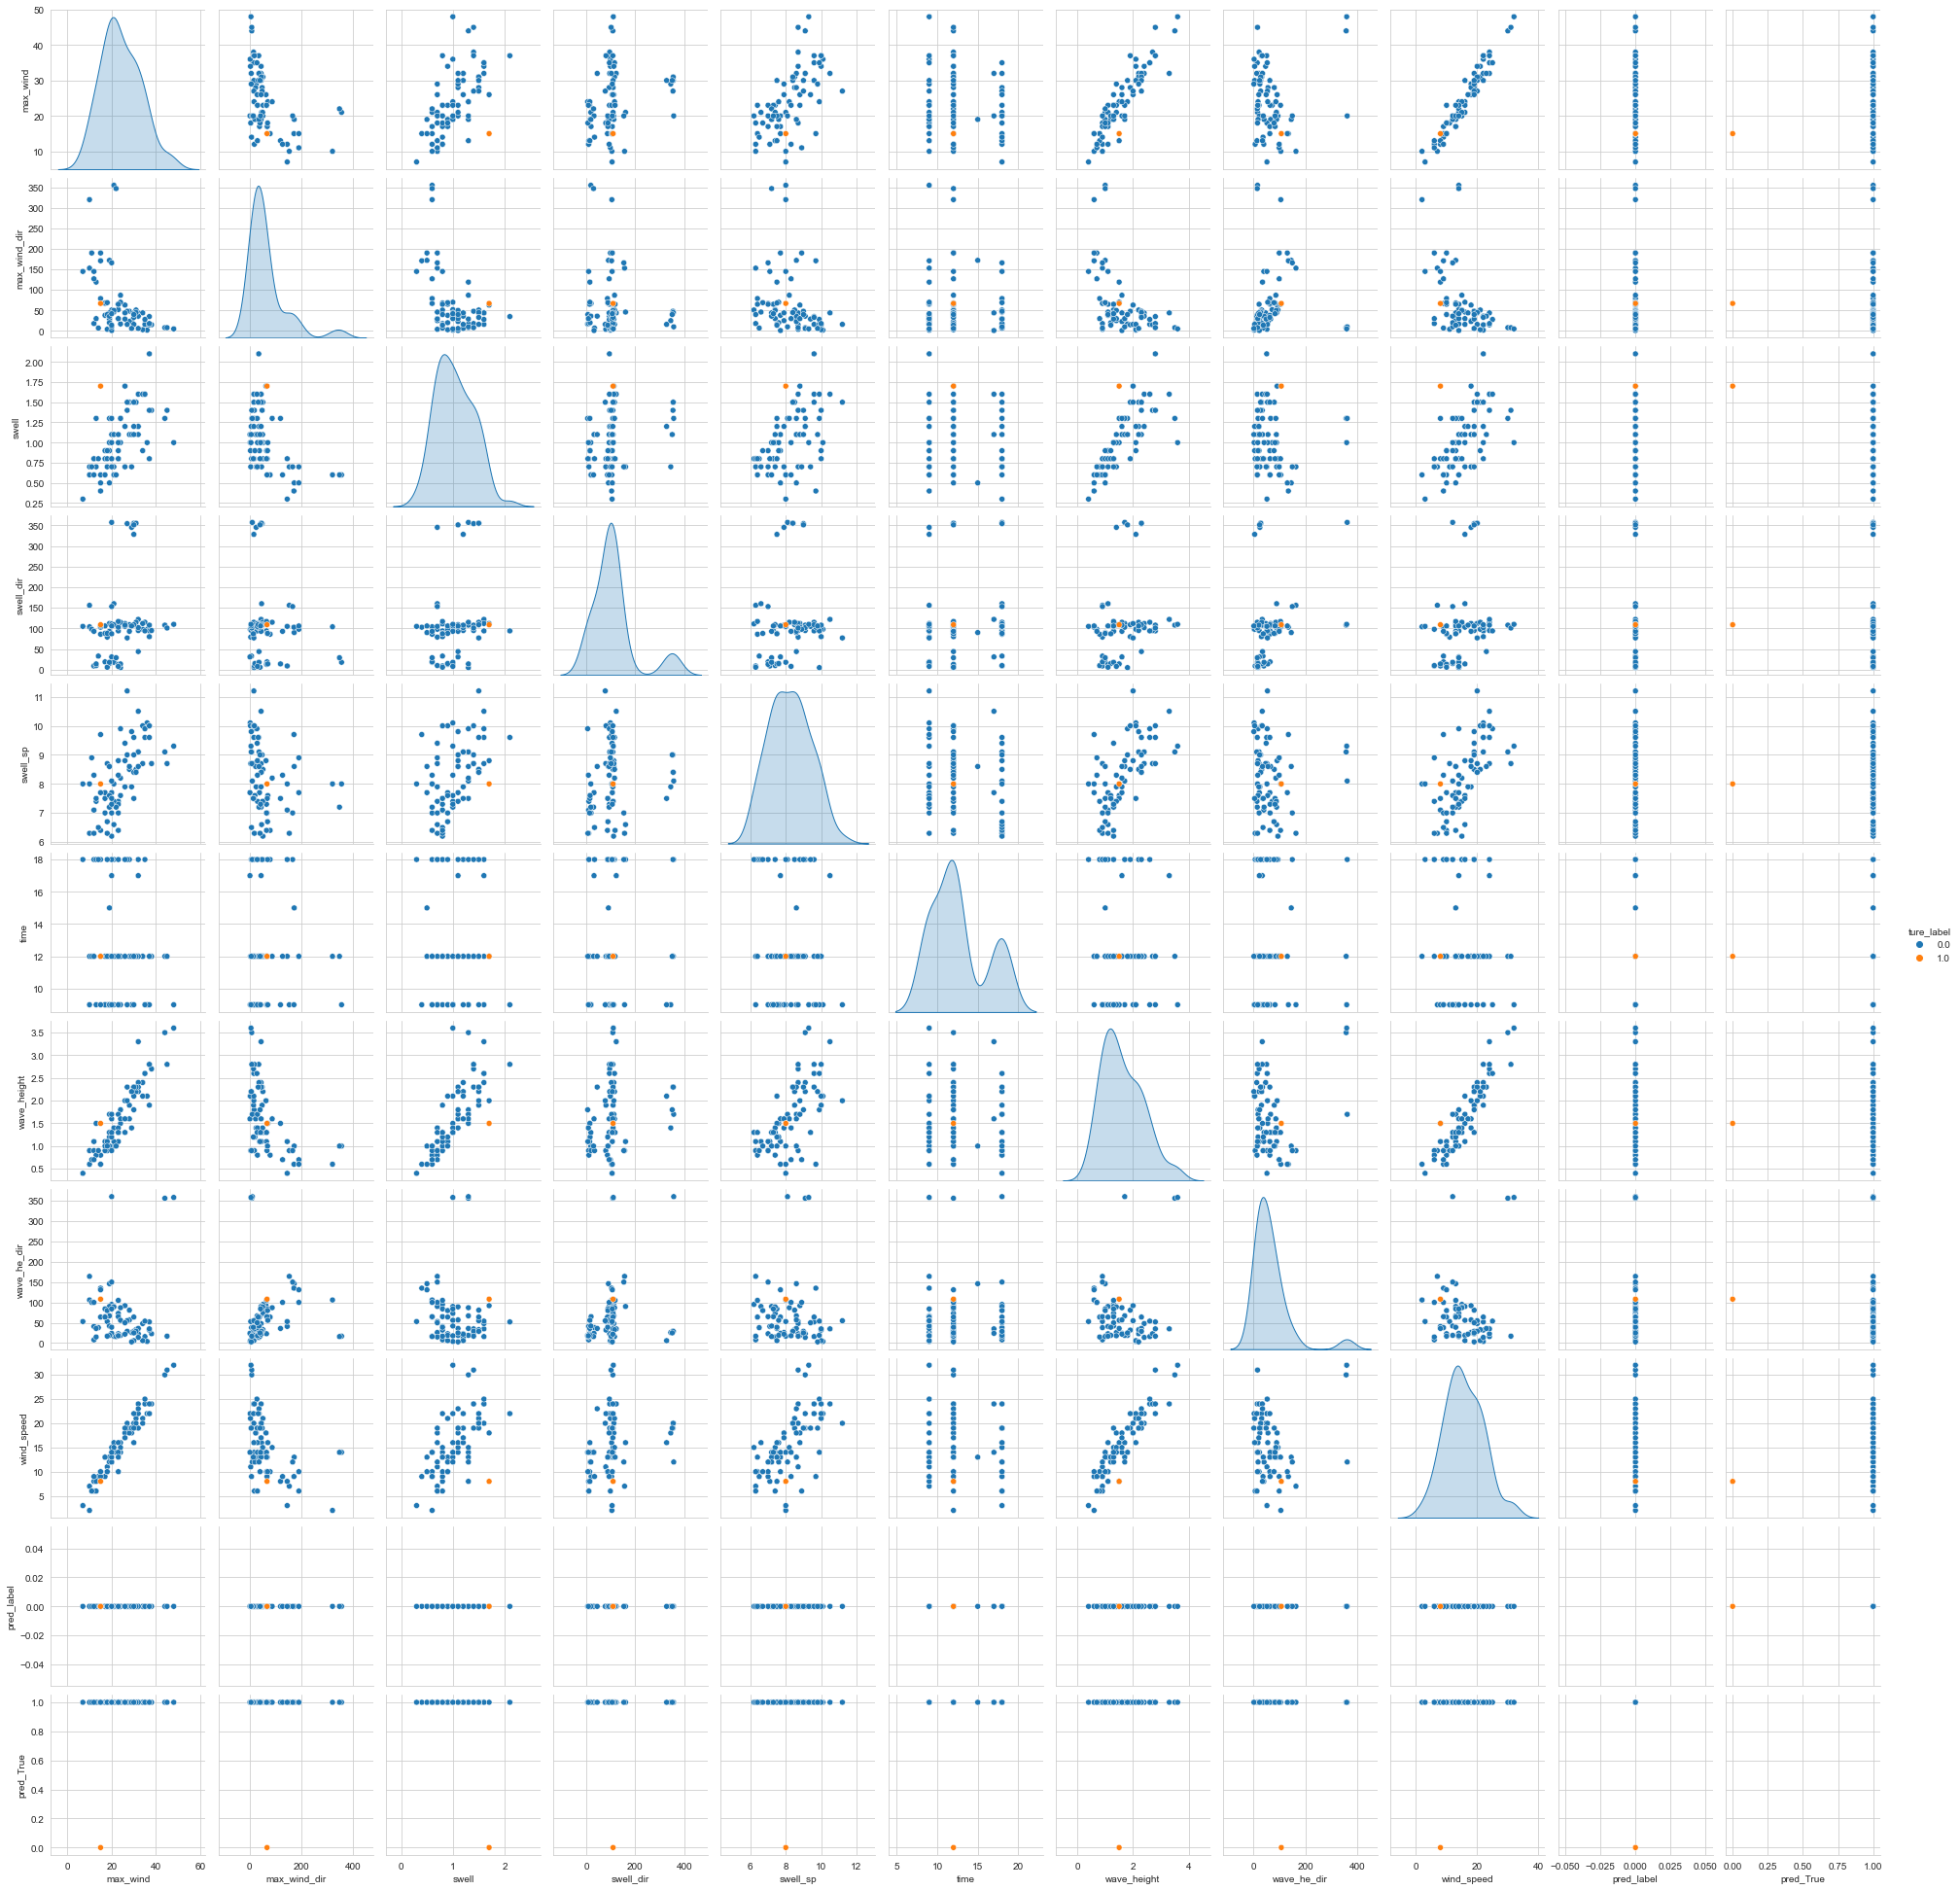
\includegraphics[keepaspectratio, scale=0.25]{fig/chapter4/kurosima_1_ture.png}
 \caption{黒島航路1日前モデルの真値ラベル別}
 \label{kurosima_1_scatter_ture}
\end{figure}

\subsection{画像データの考察}
\subsubsection{波高レイヤー画像}

表\ref{img_wave_hateruma}の波照間航路1日前モデルにおいてテストデータ予測結果の混同行列図\ref{hateruma_1_conf}となり、True labelの0は運航、1が欠航であり、Predicted labelは予想したラベルとなる。TP、FN、FP、TNの画像例として図\ref{hateruma_1_TP}、図\ref{hateruma_1_FN}、図\ref{hateruma_1_FP}、図\ref{hateruma_1_TN}がある。これらの画像からこのモデルは画像全体が青色の場合に運航と判断していることが確認できる。またその反対に画像全体と画像中心部が赤色の画像を欠航と判断していることが確認できる。FP部分の画像が運航として分類された理由として
、図\ref{hateruma_1_FP}の画像は12月24日13:00に取得された画像だが教師ラベル1日後の12月25日13:00のデータが紐づいているため12月25日13:00の画像を確認すると図\ref{hateruma_1_FP_1}となっており波照間航路線のある部分は青色が確認できる。そのため当日は運航していたと考えられ、図\ref{hateruma_1_FP}の画像の波照間航路線は赤色になっており欠航とモデルは判断したと考えられる。FN部分の画像で運航されると誤分類されているのは図\ref{hateruma_1_FN}の一枚のみであった。この画像の教師ラベル当日の時間の画像を見ると図\ref{hateruma_1_FN_1}となっており、画像は波照間行路線の部分が青色のため当日は運航でき、教師データは運航となっている。しかし、画像大部分が赤色なのでモデルは欠航と予測したと考えられる。

\begin{figure}[H]
 \centering
 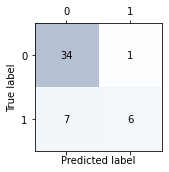
\includegraphics[keepaspectratio, scale=0.8]{fig/chapter4/wave_hateruma_1/hateruma_1_conf.png}
 \caption{波照間航路1日前モデルの混同行列}
 \label{hateruma_1_conf}
\end{figure}

\newpage

\begin{figure}[htbp]
 \begin{minipage}{0.5\hsize}
  \begin{center}
   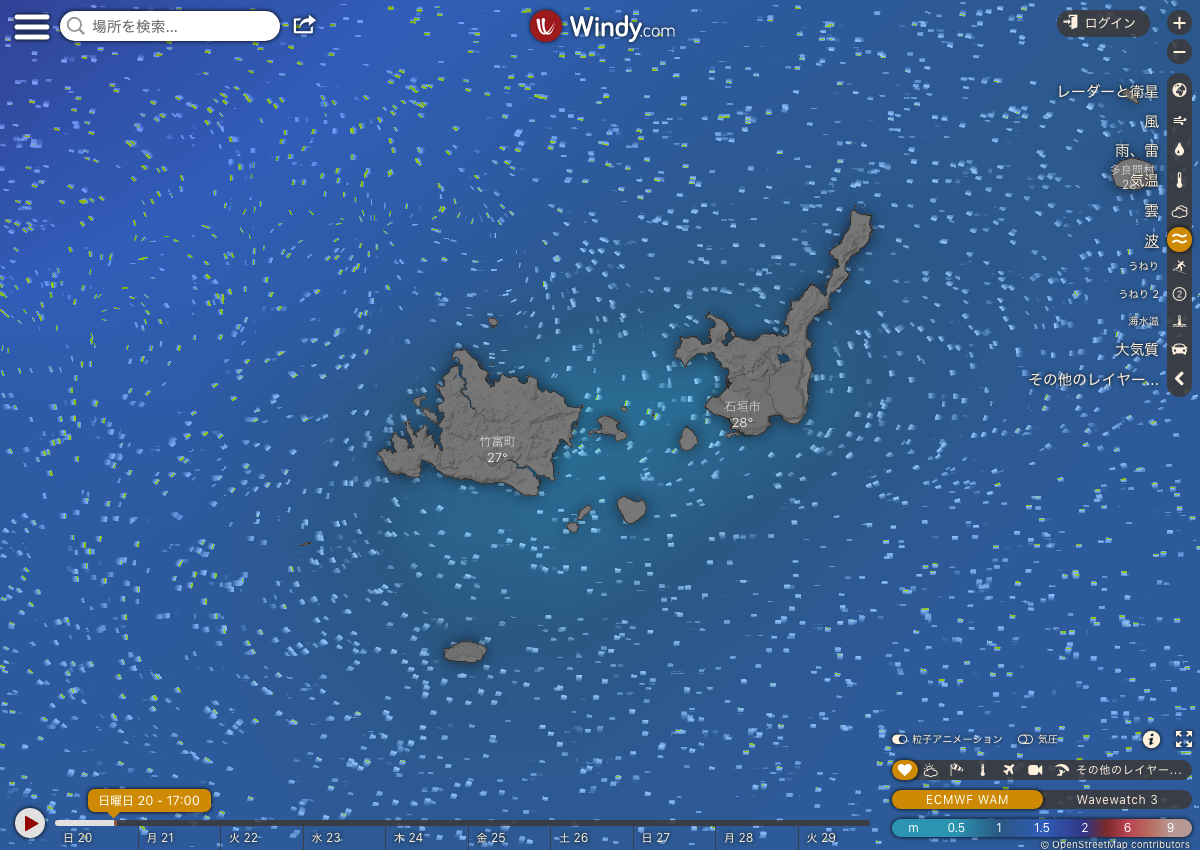
\includegraphics[keepaspectratio, scale=0.16]{fig/chapter4/wave_hateruma_1/TP.png}
   %2020-09-20_17/00_0_0.png
  \end{center}
  \caption{波照間航路1日前モデルのTP画像例}
  \label{hateruma_1_TP}
 \end{minipage}
 \begin{minipage}{0.5\hsize}
  \begin{center}
  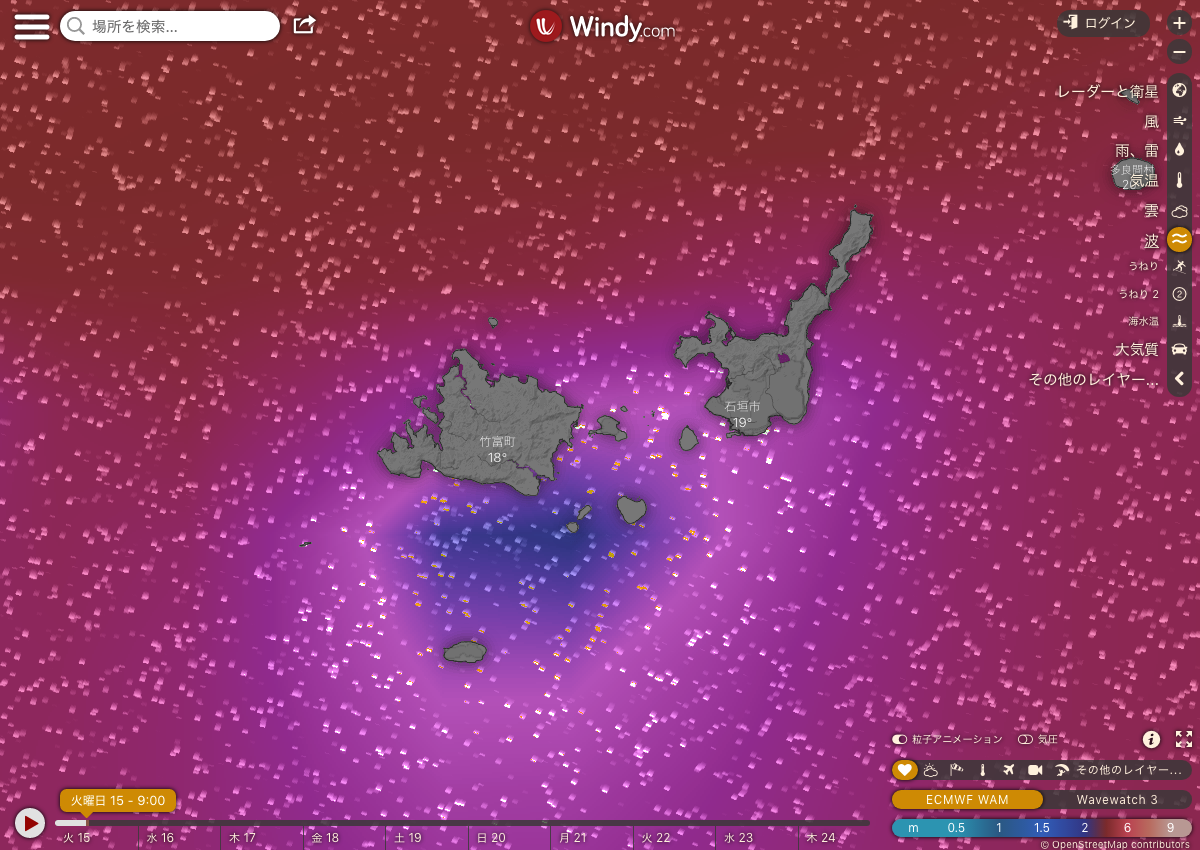
\includegraphics[keepaspectratio, scale=0.16]{fig/chapter4/wave_hateruma_1/FN.png}
  %2020-12-15 9/00_1_0
  \end{center}
   \caption{波照間航路1日前モデルのFN画像}
  \label{hateruma_1_FN}
 \end{minipage}
\end{figure}

\begin{figure}[htbp]
 \begin{minipage}{0.5\hsize}
  \begin{center}
   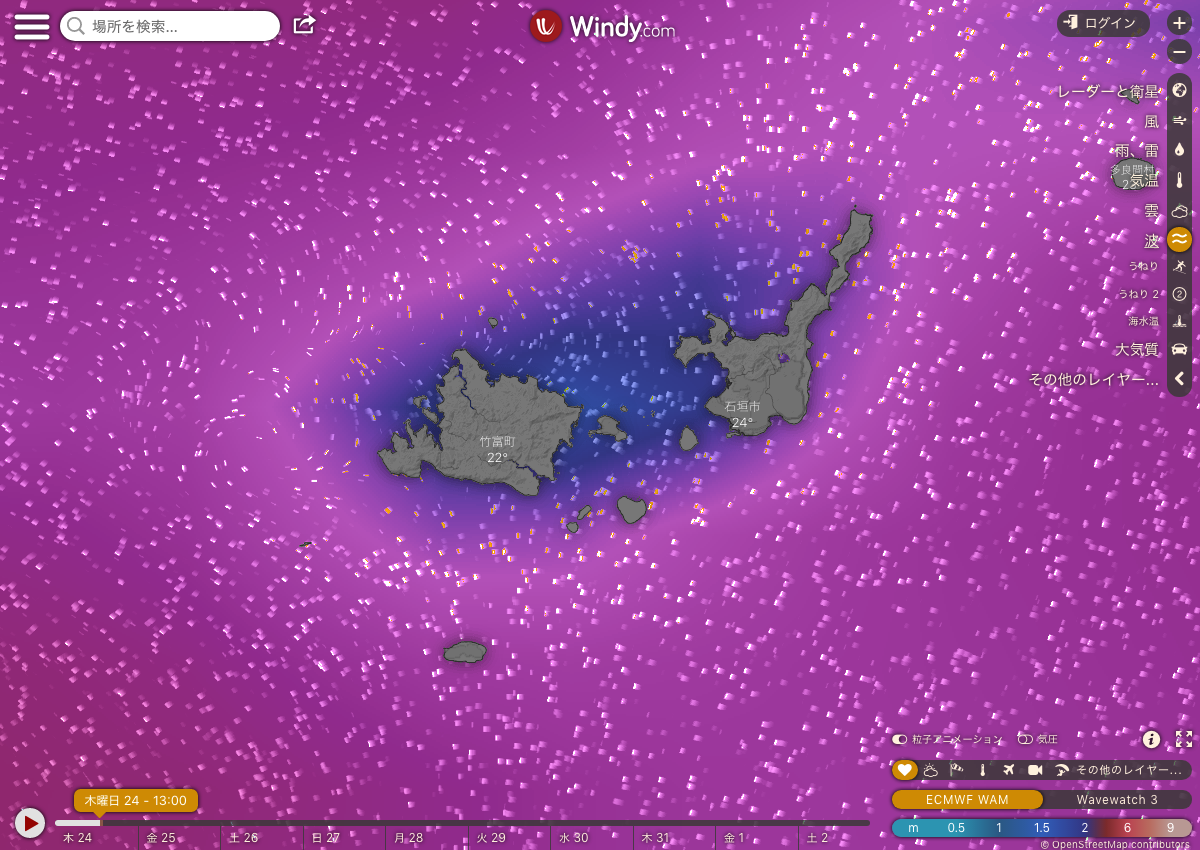
\includegraphics[keepaspectratio, scale=0.16]{fig/chapter4/wave_hateruma_1/FP.png}
   %2020-12-24 13/00/00
  \end{center}
  \caption{波照間航路1日前モデルのFP画像例}
  \label{hateruma_1_FP}
 \end{minipage}
 \begin{minipage}{0.5\hsize}
  \begin{center}
  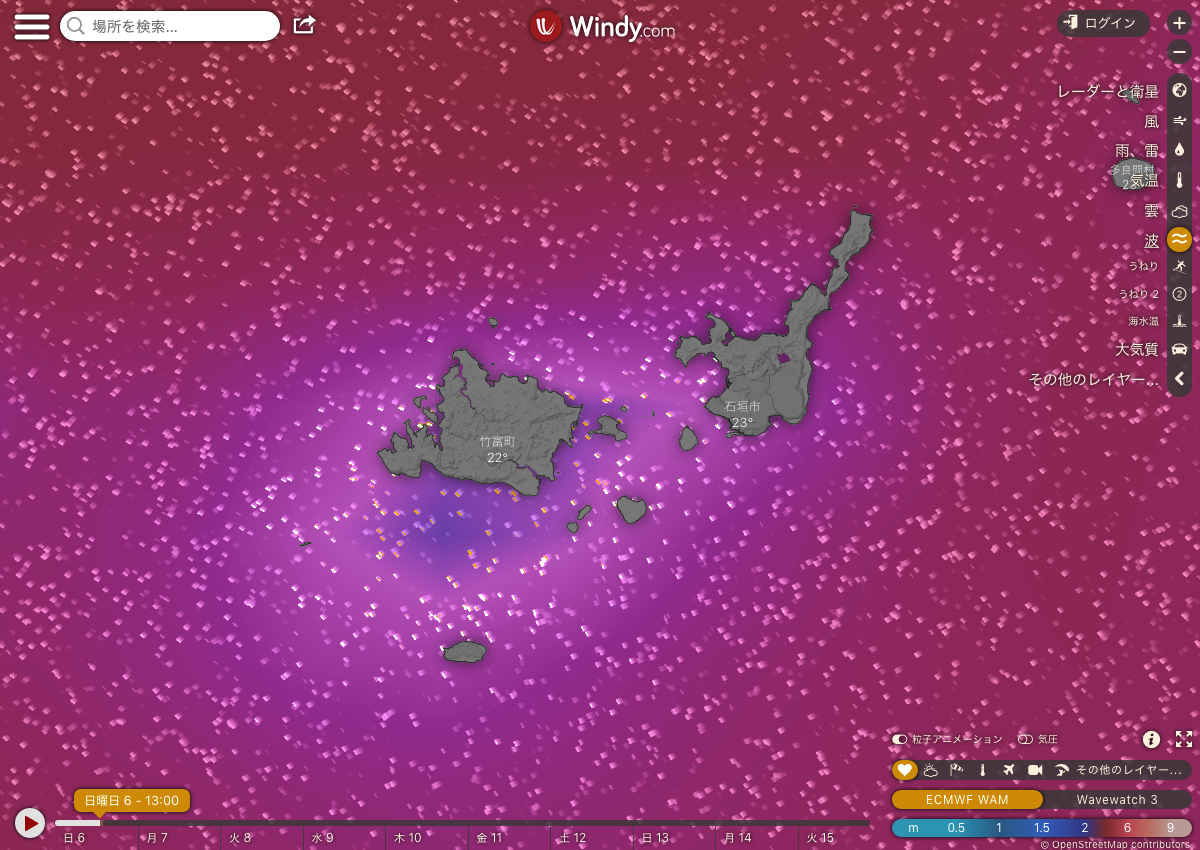
\includegraphics[keepaspectratio, scale=0.16]{fig/chapter4/wave_hateruma_1/TN.png}
  %2021-12-06 13/00_1_1.png
  \end{center}
   \caption{波照間航路1日前モデルのTN画像例}
  \label{hateruma_1_TN}
 \end{minipage}
\end{figure}

\begin{figure}[H]
 \begin{minipage}{0.5\hsize}
  \begin{center}
   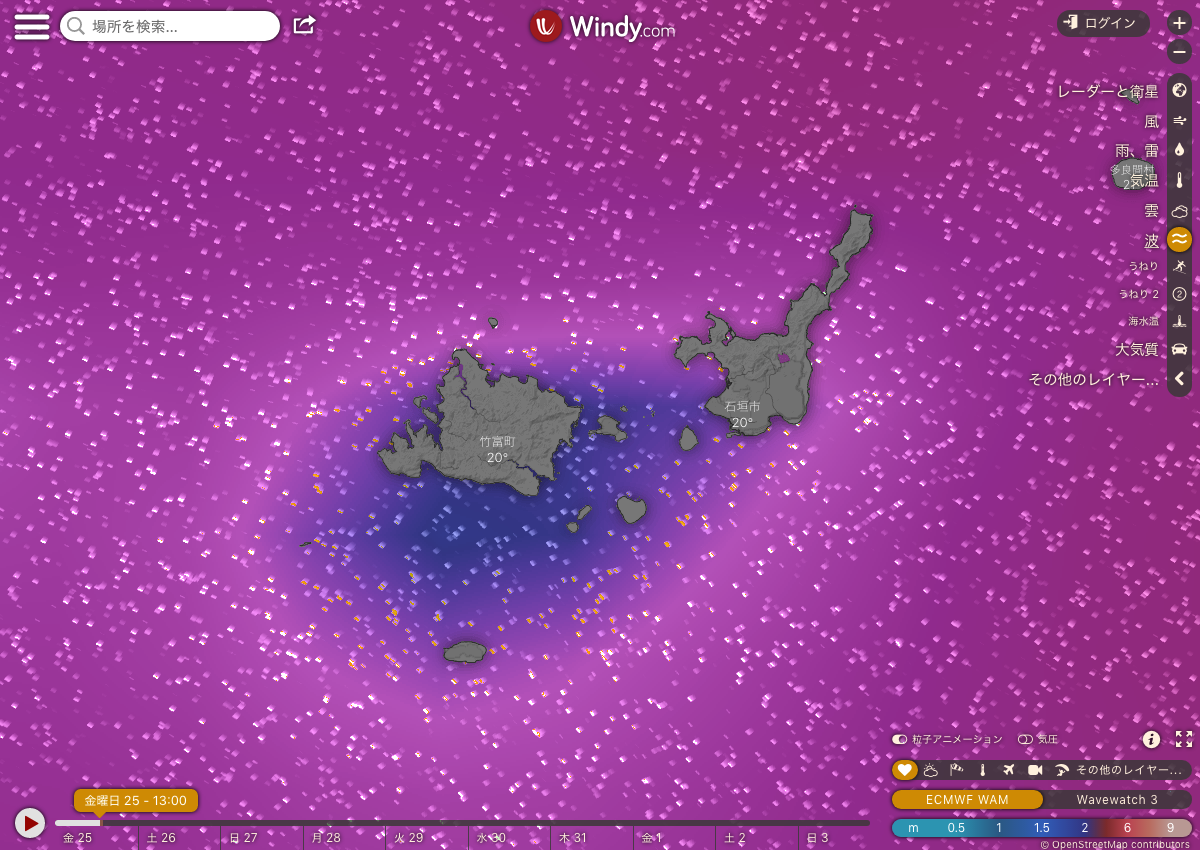
\includegraphics[keepaspectratio, scale=0.16]{fig/chapter4/wave_hateruma_1/FP_1.png}
   %2020-12-24 13/00/00
  \end{center}
  \caption{FP画像1日後の教師ラベル当日の画像}
  \label{hateruma_1_FP_1}
 \end{minipage}
 \begin{minipage}{0.5\hsize}
  \begin{center}
  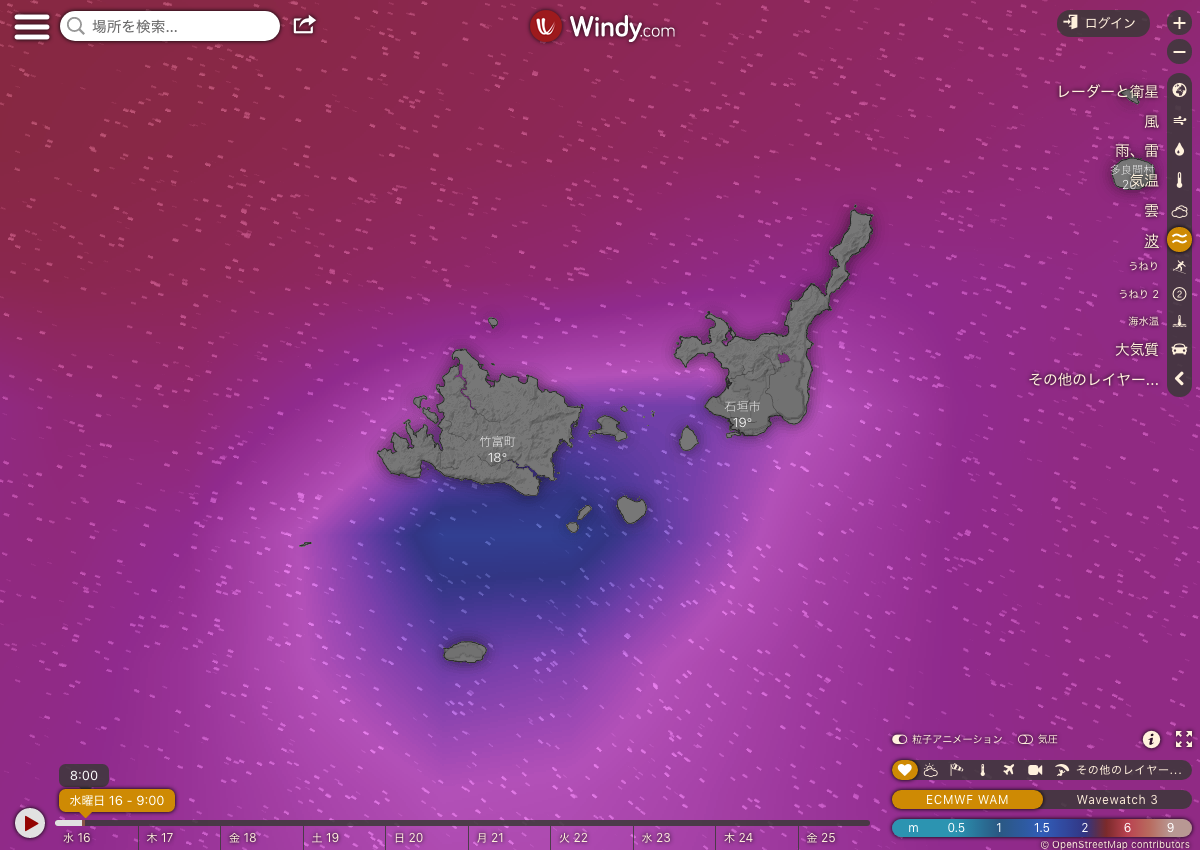
\includegraphics[keepaspectratio, scale=0.16]{fig/chapter4/wave_hateruma_1/FN_1.png}
  %2021-12-06 13/00_1_1.png
  \end{center}
   \caption{FN画像1日後の教師ラベル当日の画像}
  \label{hateruma_1_FN_1}
 \end{minipage}
\end{figure}

\newpage

表\ref{img_wave_hateruma}の波照間航路2日前モデルにおいてテストデータ予測結果の混同行列図\ref{hateruma_2_conf}となり、モデルが運航どのテストデータに対しても運航であると予測していることが確認できる。トレーニングデータを確認すると運航ラベルの付いた画像に図\ref{aka}のような画像や図\ref{unkou_ao}があることが確認できた。トレーニングデータ中の運航ラベルのついたデータが画像によって一貫性がなく、RGBの値も大きく異なるためにモデルの学習が適切に行えていないことが考えられる。%また、この航路は時間が進むに連れて教師データのが激しいため、3日前モデル以降のモデルでは全く予測できないことが考えられる。

%0 0 2021-01-01 09:50:00 ../data/now_img_scrape/wave_height/9:00/2020-12-30 09:00:00.png
%0 0 2020-09-13 13:25:00 ../data/now_img_scrape/wave_height/13:00/2020-09-1113:00:00.png

\begin{figure}[H]
 \centering
 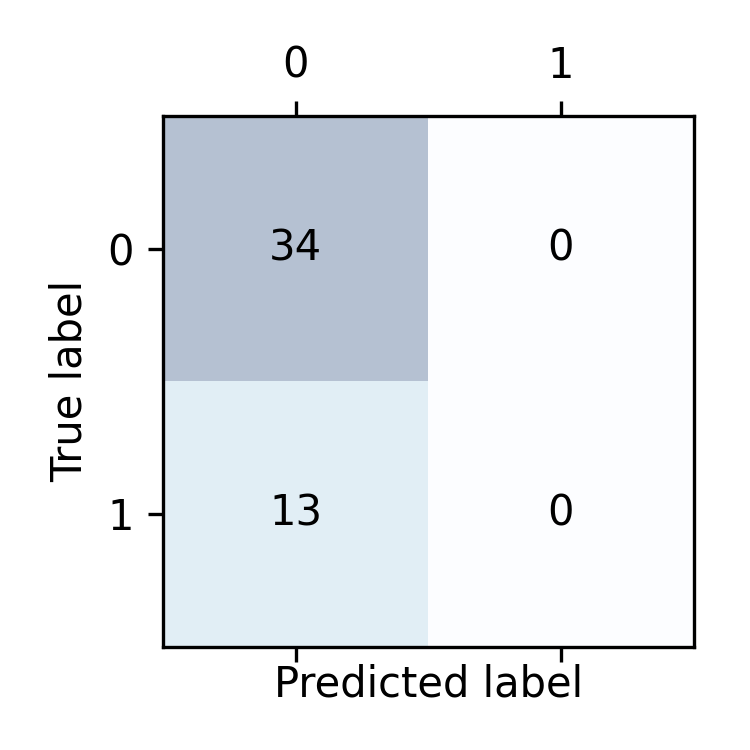
\includegraphics[keepaspectratio, scale=0.8]{fig/chapter4/wave_hateruma_2/hateruma_route_hateruma_dep_2.png}
 \caption{波照間航路2日前モデルの混同行列}
 \label{hateruma_2_conf}
\end{figure}

\begin{figure}[htbp]
 \begin{minipage}{0.5\hsize}
  \begin{center}
   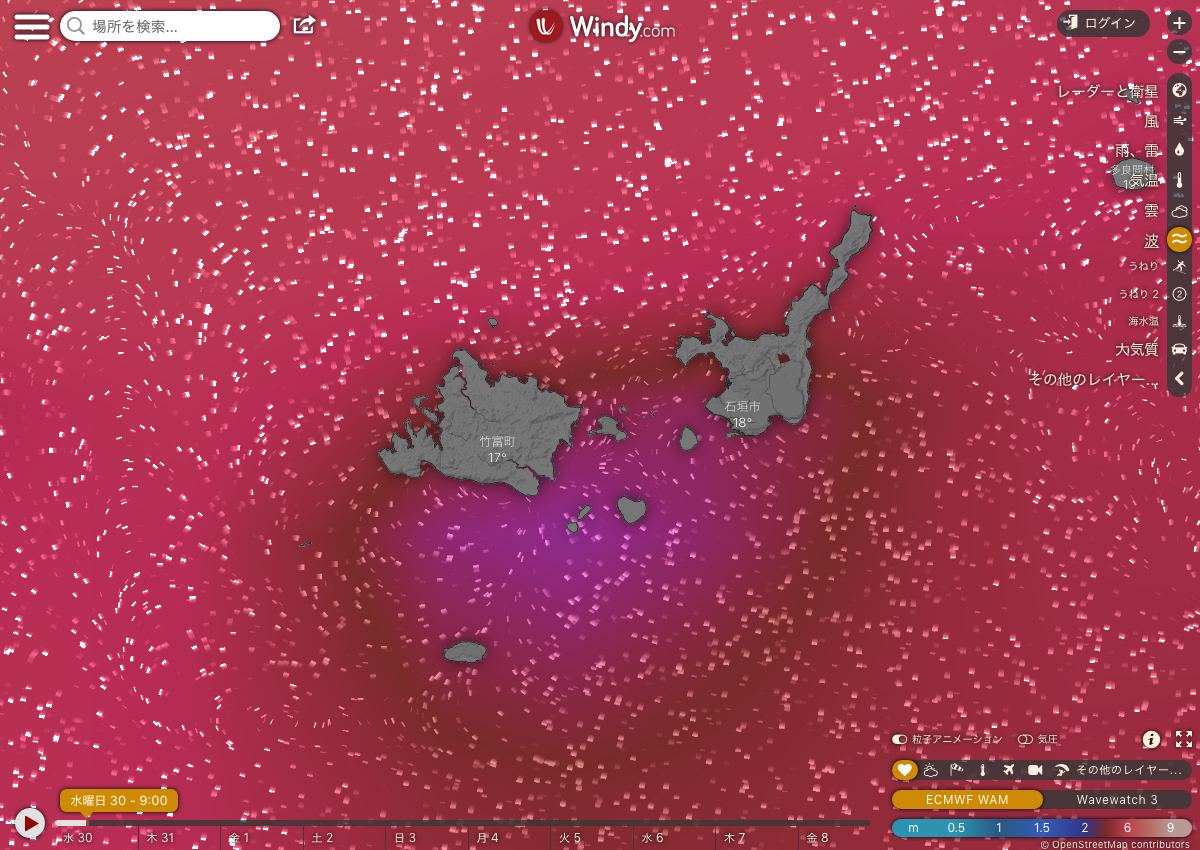
\includegraphics[keepaspectratio, scale=0.17]{fig/chapter4/wave_hateruma_2/unkou_aka.png}
   %2020-12-24 13/00/00
  \end{center}
  \caption{教師ラベル:運航 1}
  \label{aka}
 \end{minipage}
 \begin{minipage}{0.5\hsize}
  \begin{center}
  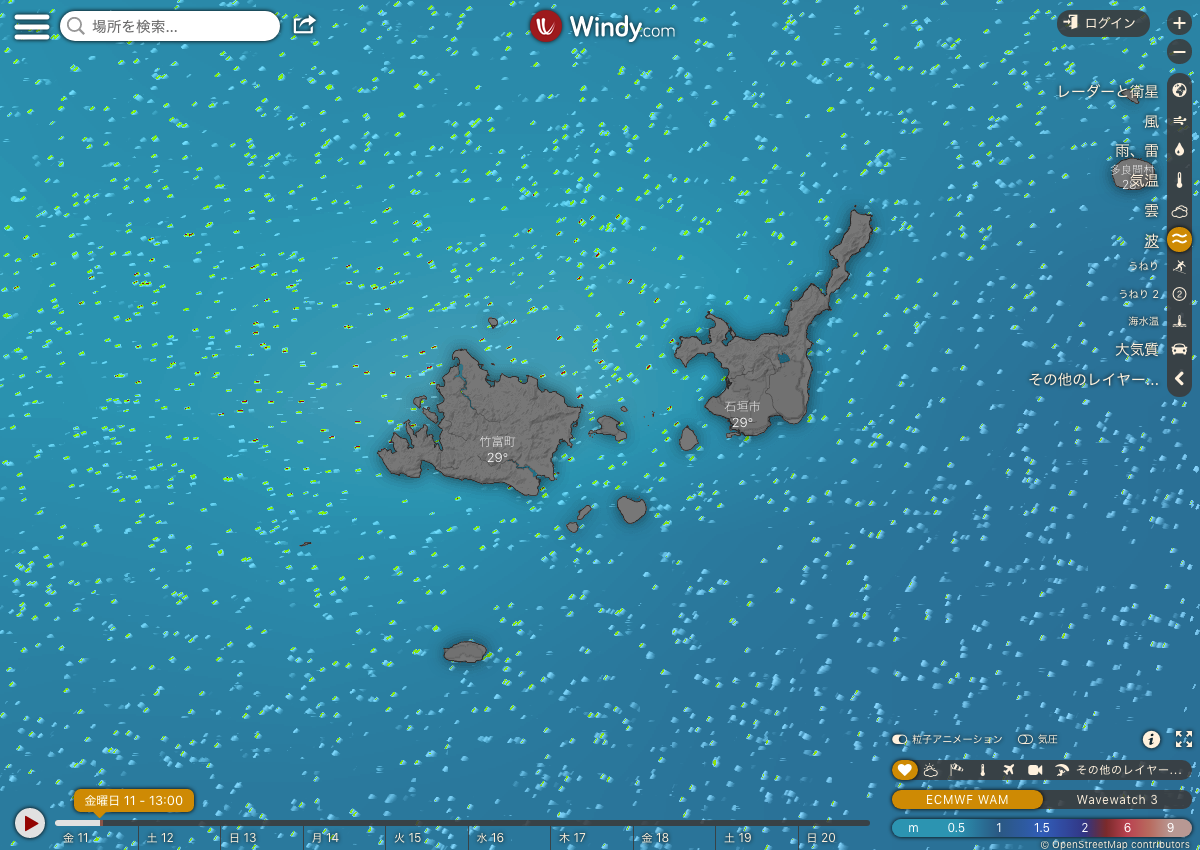
\includegraphics[keepaspectratio, scale=0.17]{fig/chapter4/wave_hateruma_2/unkou_ao.png}
  %2021-12-06 13/00_1_1.png
  \end{center}
   \caption{教師ラベル:運航 2}
  \label{unkou_ao}
 \end{minipage}
\end{figure}

表\ref{img_wave_hatoma}の波照間航路当日モデルにおいてテストデータ予測結果の混同行列図\ref{hatoma_0_conf}となり、TP、FN、FP、TNの画像例として図\ref{hatoma_0_TP}、図\ref{hatoma_0_FN}、図\ref{hatoma_0_FP}、図\ref{hatoma_0_TN}がある。FNが誤分類された理由としてトレーニングデータ中の画像として図\ref{hatoma_0_FN_setu}があり、図\ref{hatoma_0_FN}と傾向が似ているにもかかわらず教師データが欠航のため、誤分類されたと考えられる。また、傾向が似ているにもかかわらず教師データが異なる理由として、当日の状況が視程が500m以下\cite{stan}であったと考えられる。または、風速レイヤーの画像を確認すると風向きが真逆だったため、風向が原因であると考えられる。FPが誤分類された理由として、トレーニングデータ中の画像に図\ref{hatoma_0_FP_setu}が教師データが運航として学習されているために傾向の似ている図\ref{hatoma_0_FP}が誤分類されたと考えられる。
\\ モデルがn日前のnが増加するたびにF値が減少していることが確認できる。これは教師データと特徴量のデータを取得した日付が離れることに比例していると考えられる。

\begin{figure}[H]
 \centering
 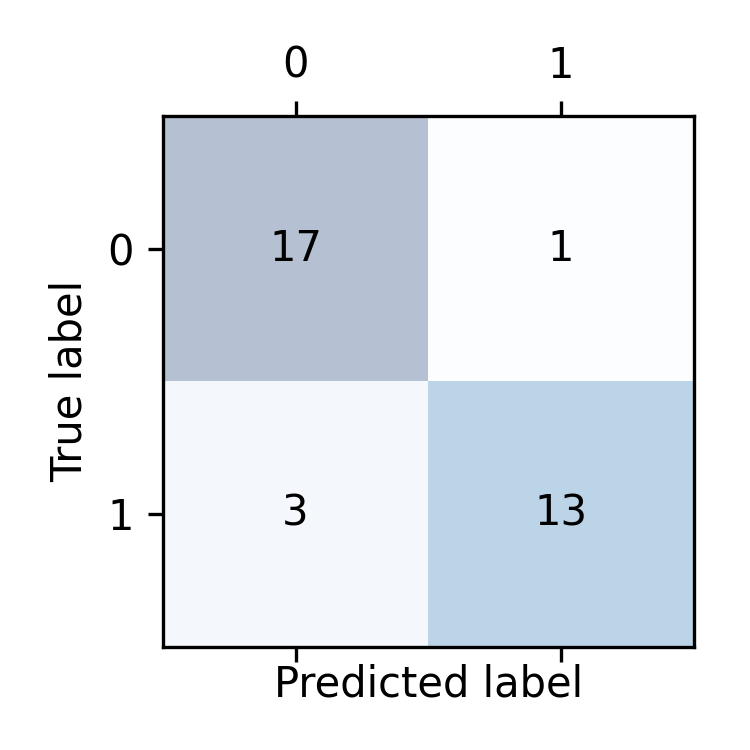
\includegraphics[keepaspectratio, scale=0.8]{fig/chapter4/wave_hatoma_0/hatoma_route_hatoma_dep_0.png}
 \caption{鳩間島航路当日モデルの混同行列}
 \label{hatoma_0_conf}
\end{figure}

\begin{figure}[htbp]
 \begin{minipage}{0.5\hsize}
  \begin{center}
   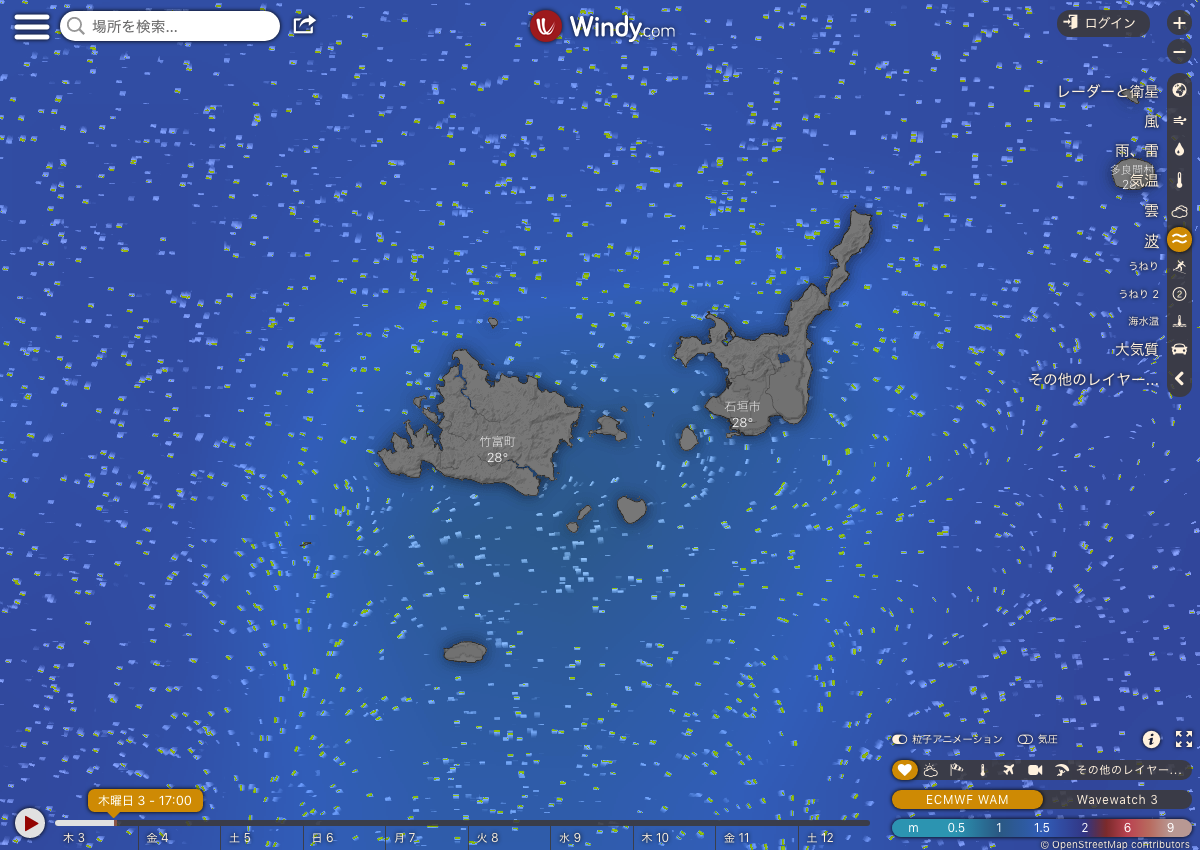
\includegraphics[keepaspectratio, scale=0.16]{fig/chapter4/wave_hatoma_0/TP.png}
   %2020-09-03 17/00/00_0_0
  \end{center}
  \caption{鳩間島航路当日モデルのTP画像例}
  \label{hatoma_0_TP}
 \end{minipage}
 \begin{minipage}{0.5\hsize}
  \begin{center}
  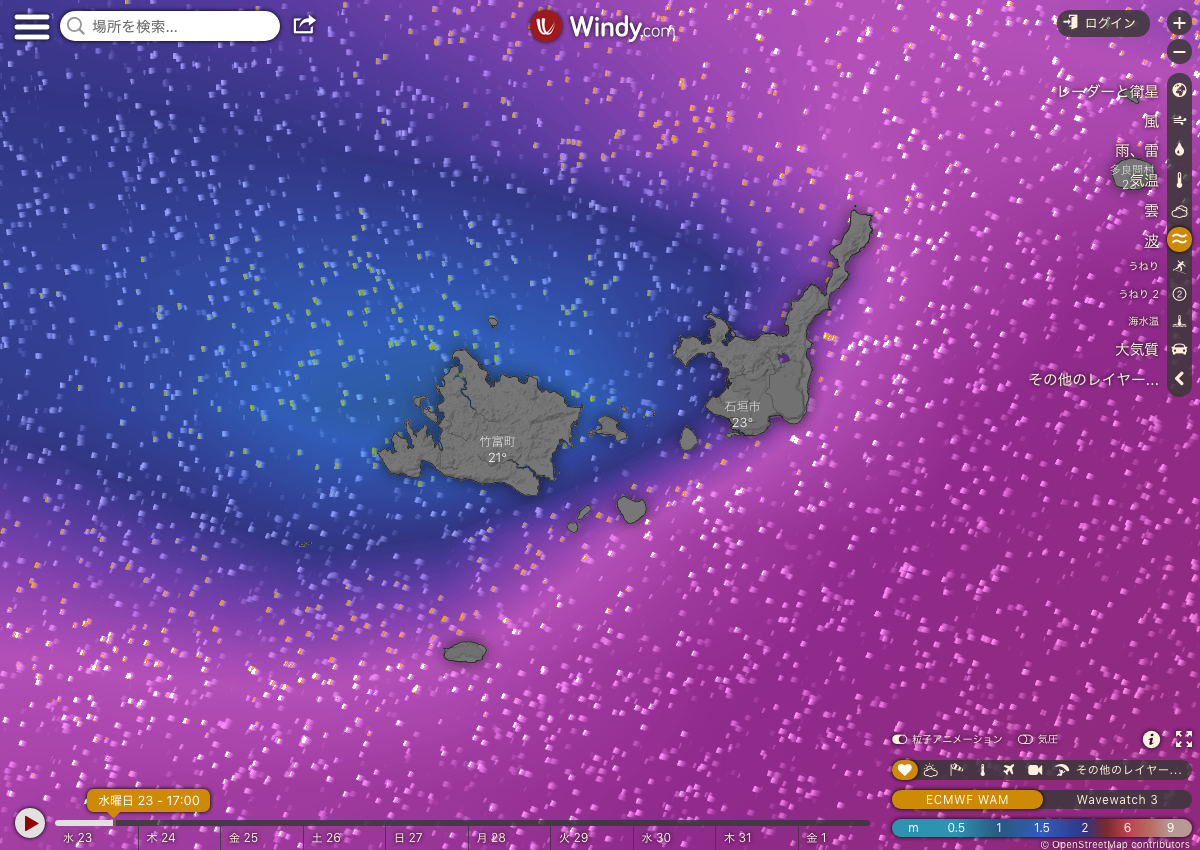
\includegraphics[keepaspectratio, scale=0.16]{fig/chapter4/wave_hatoma_0/FN.png}
   %2020-12-23 17/00/00.png
  \end{center}
   \caption{鳩間島航路当日モデルのFN画像}
  \label{hatoma_0_FN}
 \end{minipage}
\end{figure}

\begin{figure}[htbp]
 \begin{minipage}{0.5\hsize}
  \begin{center}
   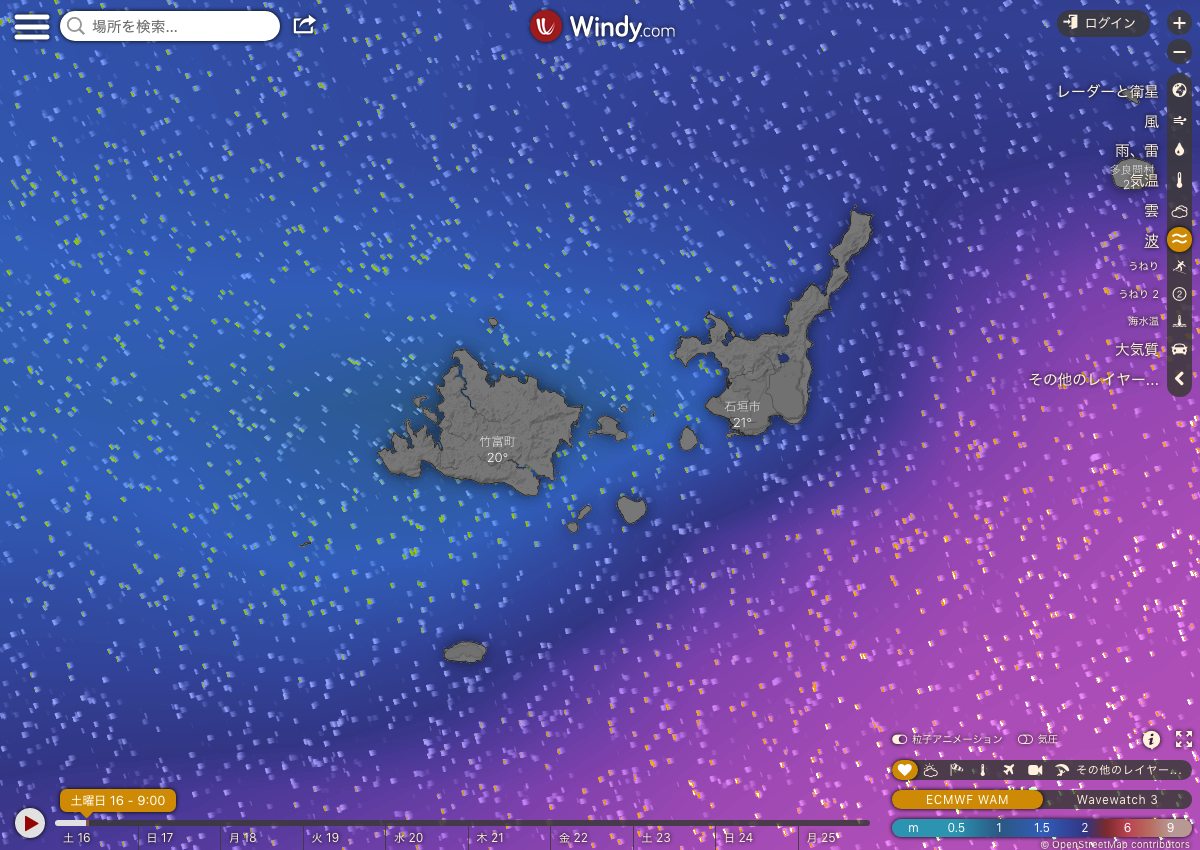
\includegraphics[keepaspectratio, scale=0.16]{fig/chapter4/wave_hatoma_0/FP.png}
   %2021-01-16 09/00/00_1_0.png
  \end{center}
  \caption{鳩間島航路当日モデルのFP画像例}
  \label{hatoma_0_FP}
 \end{minipage}
 \begin{minipage}{0.5\hsize}
  \begin{center}
  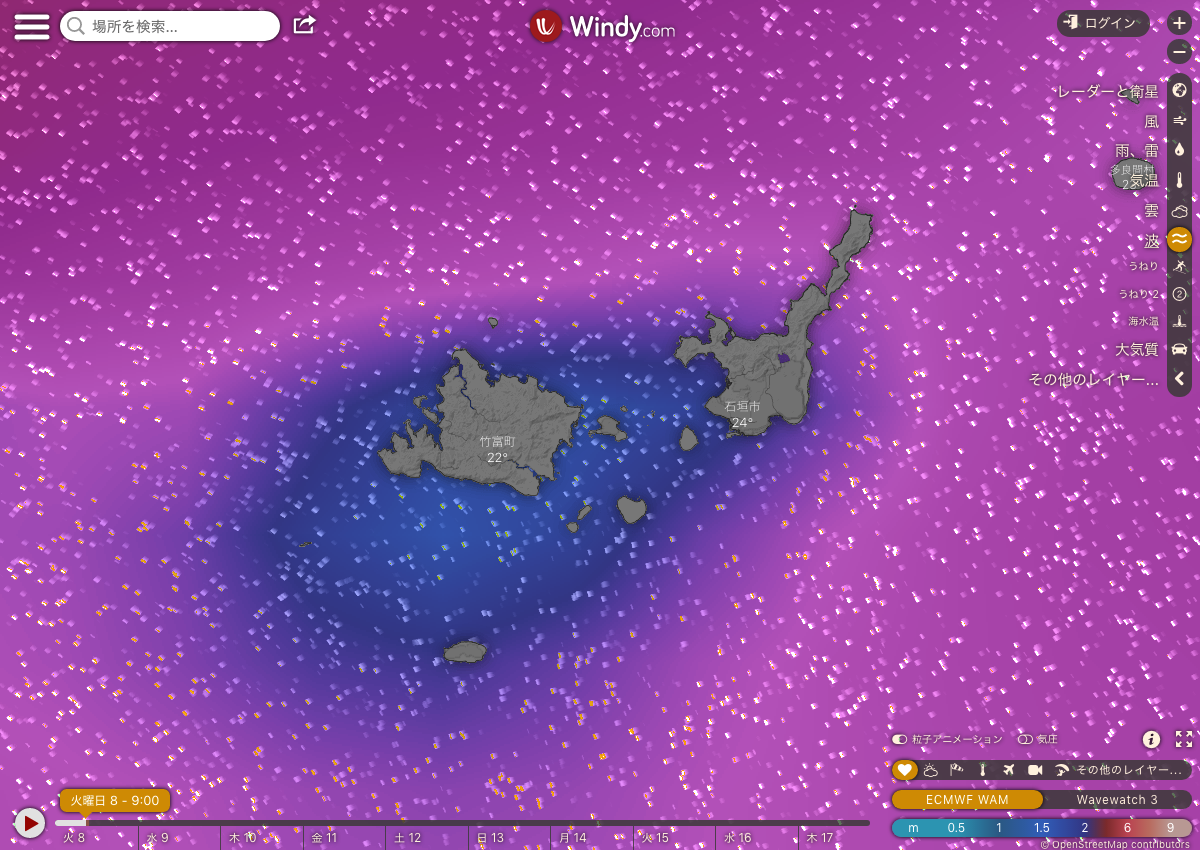
\includegraphics[keepaspectratio, scale=0.16]{fig/chapter4/wave_hatoma_0/TN.png}
  %2020-12-08 09/00/00_1_1.png
  \end{center}
   \caption{鳩間島航路当日モデルのTN画像例}
  \label{hatoma_0_TN}
 \end{minipage}
\end{figure}

\begin{figure}[H]
 \begin{minipage}{0.5\hsize}
  \begin{center}
   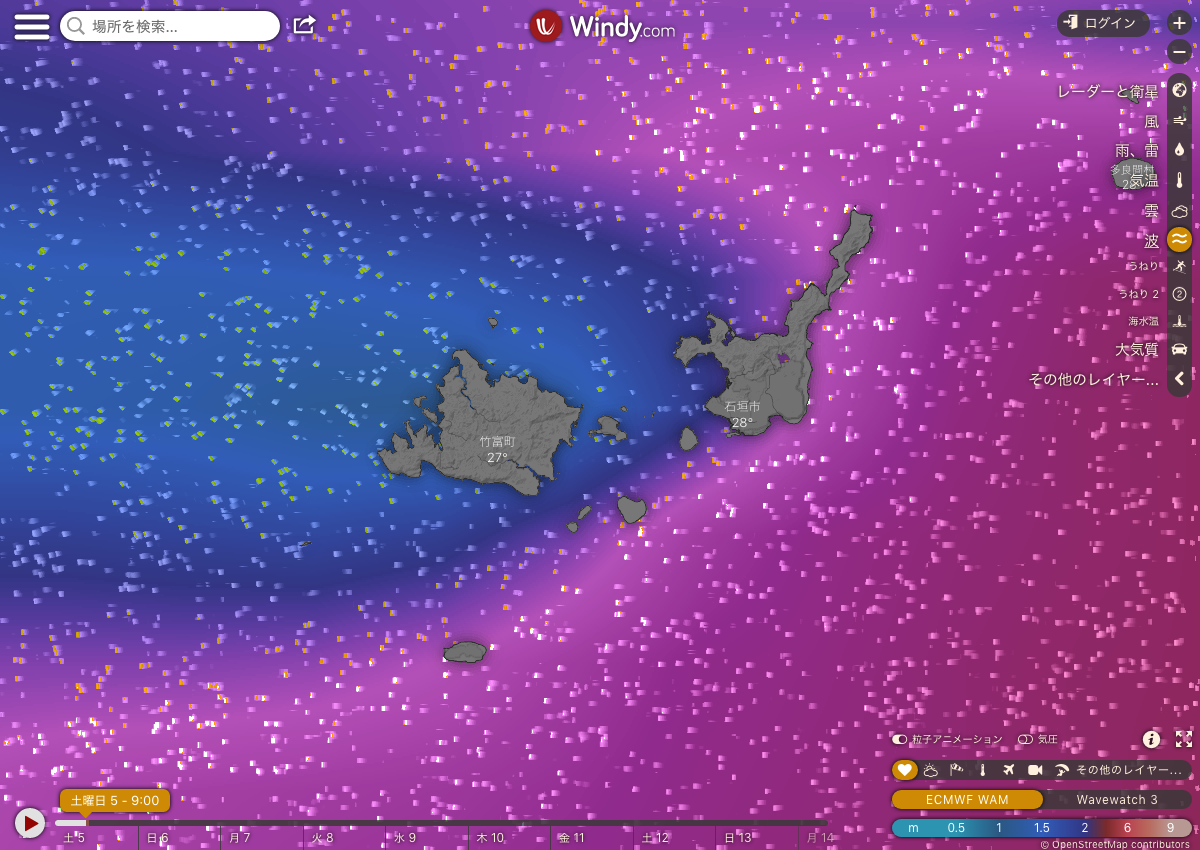
\includegraphics[keepaspectratio, scale=0.16]{fig/chapter4/wave_hatoma_0/FN_setu.png}
   %2020-09-05 09/00/00_FN_setu.png
  \end{center}
  \caption{教師ラベル:欠航}
  \label{hatoma_0_FN_setu}
 \end{minipage}
 \begin{minipage}{0.5\hsize}
  \begin{center}
  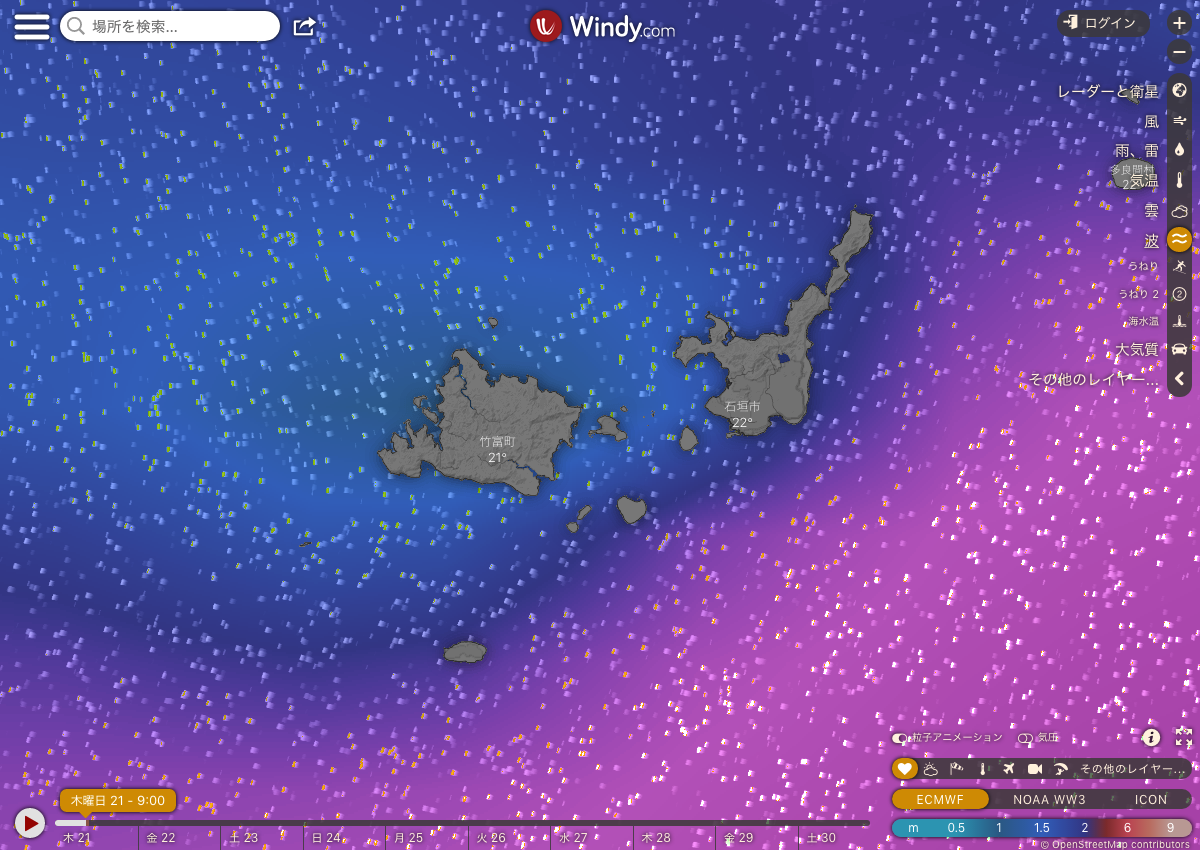
\includegraphics[keepaspectratio, scale=0.16]{fig/chapter4/wave_hatoma_0/unkou_FP_setu.png}
   %2021-01-21 09/00/00_unkou_FP_setu.png
  \end{center}
   \caption{教師ラベル:運航}
  \label{hatoma_0_FP_setu}
 \end{minipage}
\end{figure}

表\ref{img_wave_taketomi}の竹富航路では全てのモデルにおいてF値が0.000となっている。これは表\ref{img_wave_hateruma}の2日前モデルと同じ理由である。また、竹富航路が欠航データの極端に少ない航路であり、欠航データの学習不足の状態となっていると考えられる。

\subsubsection{風速レイヤー画像}

表\ref{img_wind_hateruma}の波照間航路1日前モデルにおいてテストデータ予測結果の混同行列図\ref{wind_hateruma_1_conf}となる。波高レイヤーの表\ref{img_wave_hateruma}の1日前モデル考察と同じように風速レイヤーでも同様の傾向が見られた。
\\ 2日前モデルの混同行列図\ref{wind_hateruma_2_conf}となり、2日前モデル以降でも波高レイヤーの表\ref{img_wave_hateruma}の2日前と同様の傾向が見られたため学習モデルがうまく学習できていないと考えられる。

\begin{figure}[H]
 \begin{minipage}{0.5\hsize}
  \begin{center}
   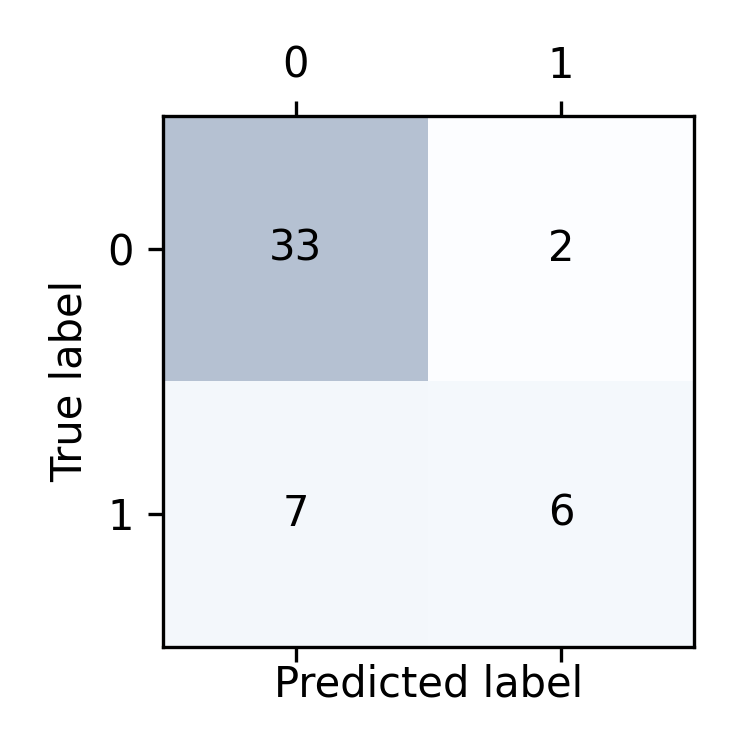
\includegraphics[keepaspectratio, scale=0.5]{fig/chapter4/wind_hateruma_1/hateruma_route_hateruma_dep_1.png}
   %2020-09-05 09/00/00_FN_setu.png
  \end{center}
  \caption{波照間航路1日前モデルの混同行列}
  \label{wind_hateruma_1_conf}
 \end{minipage}
 \begin{minipage}{0.5\hsize}
  \begin{center}
  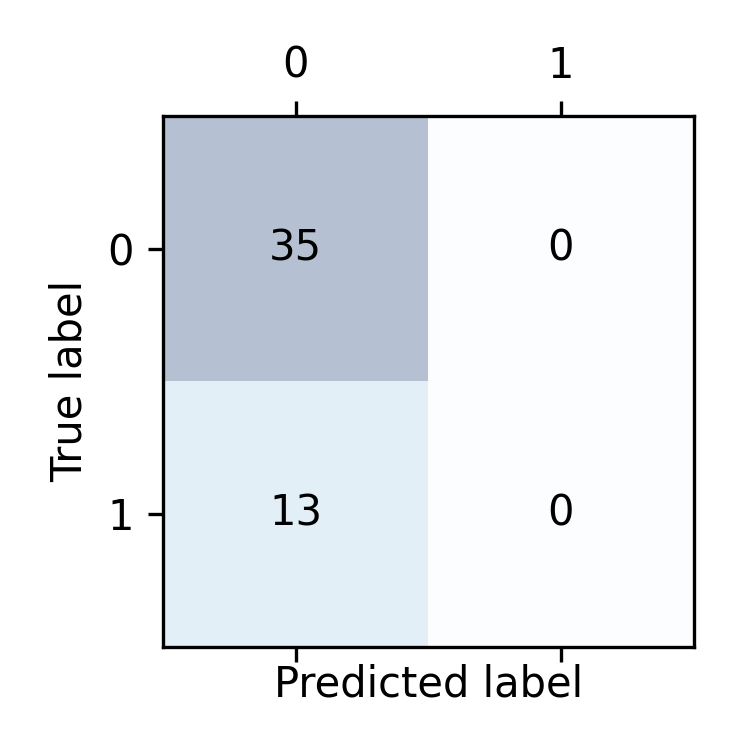
\includegraphics[keepaspectratio, scale=0.5]{fig/chapter4/wind_hateruma_2/hateruma_route_hateruma_dep_2.png}
   %2021-01-21 09/00/00_unkou_FP_setu.png
  \end{center}
   \caption{波照間航路2日前モデルの混同行列}
 \label{wind_hateruma_2_conf}
 \end{minipage}
\end{figure}

表\ref{img_wind_iriue}の西表上原航路は表\ref{img_wave_hatoma}と同様の傾向が見られた。またこれらの同様な傾向の見られた航路では8日前からF値の評価が7日前と比較して上昇していることが確認できる。8日間というスパンが教師データと画像をうまく一致するような傾向が本研究で対象とした航路に存在すると考えられる。

表\ref{img_wind_taketomi}の竹富航路でも波高レイヤーと同様に欠航データが極端に少ないため精度が良くならないことが確認できる。

\section{考察まとめ}
数値データでは、散布図により特徴量と予測ラベルの分布を示すことで、モデルの重要視している特徴量を発見できた。予測精度の悪いモデルをでは、特徴量の分布に運航時と欠航時の差異がみられない。これらは教師ラベルと特徴量の取得時間のラグがあることに起因すると考えられる。波高、風速画像ではモデルの出力した予測と入力した画像、トレーニングした画像を比較することで、その航路のモデルにおける画像と教師ラベルの関係性、特徴を解析することができた。性能が極端に低いモデルではトレーニングに使用した画像において、教師ラベルと画像の特徴に規則性がほぼ無いために、画像の特徴を捉えられなかったと考えられる。風速、波高の画像どちらもモデルに対しての影響が似ていた。これは船舶の欠航が波高の高さ、風速の大きさによって決定するためであると考えられる。また、画像モデルにおいて欠航データが十分にある航路、表\ref{img_wave_hatoma}と表\ref{img_wind_iriue}では、8日前モデルからは評価指標が上昇した。これは本研究で扱った八重山諸島の周辺の気象画像と教師データの関係性において周期性があると考察できる。
\\ これらの考察より欠航予測のための数値データ、画像データの特徴抽出は時系列を考慮したデータが望ましく、つまり予測に周期性を加味できればより高い精度の予測ができるだろう。
%その航路において周期性の情報も加味されたデータセット作成が必要である。考察できる、つまり






% 今後の課題
\chapter{結論}

\section{まとめ}
本研究では船舶の運行状況が当日にしか公表されないという問題を機械学習を用い、比較的安易に入手可能な気象状況の値や気象予報図を適用し数日先までを予測する実験を実施した。画像、数値データどちらも9日先までの予測実験を行い、数値用いた予測では特徴量と教師ラベルとの関係を明らかにすることで、学習モデルが重要視している特徴を確認することができた。特徴量の分散をみることで運航データと欠航データとの特徴量の相関を確認し、予測を行うことにおいて重要な特徴量を確認することができた。画像を用いた予測では航路ごとの入力画像を確認することで、どのような画像がモデルに対して影響を与えているかを示した。また、画像分類では鳩間島、西表上原航路において当日から7日前モデルまでは評価指標が減少する傾向にあったが8日前モデルから上昇することを発見した。また、これらの考察から数値、画像データを時系列的に扱うことで特徴の変遷を保持することができると考えられる。

\section{今後の課題}
数値と画像どちらのデータも特徴があり、一方だけで無く両方のデータを活用することでデータの特徴生かしたモデル、データセットを構築することで予測精度向上が期待できるのではないかと考えた。

% 参考文献
% 参考文献
\def\line{−\hspace*{-.7zw}−}

\begin{thebibliography}{99}
%\bibitem{*}内の * は各自わかりやすい名前などをつけて、
%論文中には \cite{*} のように使用する。
%これをベースに書き換えた方が楽かも。
%書籍、論文、URLによって若干書き方が異なる。
%URLを載せる人は参考にした年月日を最後に記入すること。


%\bibitem{hoge}
%hoge
% 背景と目的のところ
\bibitem{earth}IPCC, de Coninck, H., A. Revi, M. Babiker, P. Bertoldi, M. Buckeridge, A. Cartwright, W. Dong, J. Ford, S. Fuss, J.-C. Hourcade, D. Ley, R. Mechler, P. Newman, A. Revokatova, S. Schultz, L. Steg, and T. Sugiyama, 2018: Strengthening and Implementing the Global Response. In: Global Warming of 1.5°C. An IPCC Special Report on the impacts of global warming of 1.5°C above pre-industrial levels and related global greenhouse gas emission pathways, in the context of strengthening the global response to the threat of climate change, sustainable development, and efforts to eradicate poverty [MassonDelmotte,V., P. Zhai, H.-O. P\"{o}rtner, D. Roberts, J. Skea, P.R. Shukla, A. Pirani, W. Moufouma-Okia, C. P\'{e}an, R. Pidcock, S. Connors, J.B.R. Matthews, Y. Chen, X. Zhou, M.I. Gomis, E. Lonnoy, T. Maycock, M. Tignor, and T. Waterfield (eds.)]. 
\bibitem{Related-Research1} 笹 健児,一寺田 大介,永井 紀彦,河合 弘泰,``船体運動と沿岸波浪に基づくフェリー欠航の判断基準に関する検討'',日本航海学会論文集, 120号, pp.99-106, 2009.
\bibitem{Related-Research2} Shreya Agrawal, Luke Barrington, Carla Bromberg, John Burge, Cenk Gazen, and Jason Hickey, ``Machine learning for precipitation nowcasting from radar images'', arXiv preprint arXiv:1912.12132, 2019.
\bibitem{rainfull}Using Machine Learning to "Now-cast" Precipitation in High Resolution. \url{https://ai.googleblog.com/2020/01/using-machine-learning-to-nowcast.html}
\\最終閲覧日:2021/2/1
\bibitem{nowphas} ナウファス. https://www.mlit.go.jp/kowan/nowphas/ \\最終閲覧日:2020/9/14
\bibitem{anei} 安栄観光. http://www.aneikankou.co.jp/ \\最終閲覧日:2021/1/30
\bibitem{windy}windy.com. \url{https://www.windy.com/} \\最終閲覧日:2021/1/30
\bibitem{stan}安栄観光,安全管理規定,旅客船. \\ \url{http://www.aneikankou.co.jp/res/pc/pdf/company/legal/anzenkanri5.pdf} \\最終閲覧日:2020/9/14
\bibitem{optical-flow}David J. Fleet and Y. Weiss, ``Optical flow estimation'', In Handbook of Mathematical Models in Computer Vision, 2006.
\bibitem{persistence}S. Pulkkinen, D. Nerini, A. A. P\'{e}rez Hortal, C. Velasco-Forero, A. Seed, U. Germann, and L. Foresti. Pysteps: an open-source python library for probabilistic precipitation nowcasting (v1.0). Geoscientific Model Development, 12(10):4185-4219, 2019.
\bibitem{MRMA}Jian Zhang, Kenneth Howard, Carrie Langston, Brian Kaney, Youcun Qi, Lin Tang, Heather Grams, Yadong Wang, Stephen Cocks, Steven Martinaitis, Ami Arthur, Karen Cooper, Jeff Brogden, and David Kitzmiller. ``Multi-radar multi-sensor (mrms) quantitative precipitation estimation: Initial operating capabilities'', Bulletin of the American Meteorological Society, 97(4):621-638, 2016.
\bibitem{HRRR}Stanley G. Benjamin, Stephen S. Weygandt, John M. Brown, Ming Hu, Curtis R. Alexander, Tatiana G. Smirnova, Joseph B. Olson, Eric P. James, David C. Dowell, Georg A. Grell, Haidao Lin, Steven E. Peckham, Tracy Lorraine Smith, William R. Moninger, Jaymes S. Kenyon, and Geoffrey S. Manikin, ``A north american hourly assimilation and model forecast cycle: The rapid refresh''. Monthly Weather Review, 144(4):1669-1694, 2016.
%chapter2
\bibitem{Yann LeCun}Y. LeCun, L. Bottou, Y. Bengio, and P. Haffner, ``Gradient- based learning applied to document recognition'', Proceed-ings of the IEEE, 86(11):2278-2324, 1998. 
%chapter4


\end{thebibliography}




% 謝辞
\chapter*{謝辞}
\thispagestyle{empty}

%基本的な内容は以下の通り.参考にしてみて下さい.
%厳密な決まりは無いので,個々人の文体でも構わない.
%GISゼミや英語ゼミに参加した人はその分も入れておく.
%順番は重要なので気を付けるように.(提出前に周りの人に確認してもらう.)

\hspace{1zw}
本研究の遂行、また本論文の作成にあたり、御多忙にも関わらず終始懇切なる御指導と御教授を賜わりました當間愛晃准教授に深く感謝したします。また一年間共に研究を行 い、暖かな気遣いと励ましをもって支えてくれた當間研究室の津波君、松本君、島袋君、具志堅君並びに同研究室先輩方の茂島さん、佐藤さん、伊藤さん、上原さんに感謝致します。

\begin{flushright}
 2021年 3月 \\ 大城紳之亮
\end{flushright}




% 付録
%\input{appendix.tex}

\end{document}
